%%%%%%%%%%%%%%%%%%%%%%%%%%%%%%%%%%%%%%%%%%%%%%%%%%%%%%%%%%%%%%%%%%%%%%
%  Run mode: XeLaTeX
% !TeX program = xelatex
%  !Mode: "Tex:Utf-8"
%  Authors: Xiangdong Jia
%  Date: Last Updated May-30-2023 (migrated to XeLaTeX)
%  Copyright UWC&IoT@NWNU
%%%%%%%%%%%%%%%%%%%%%%%%%%%%%%%%%%%%%%%%%%%%%%%%%%%%%%%%%%%%%%%%%%%%%%
\def\usewhat{xelatex}                               % 编译方式 xelatex
% 项目已整体迁移到 XeLaTeX，编译链：xelatex → bibtex → xelatex → xelatex
%\setlength{\baselineskip}{20pt}
%\setlength{\headheight}{25pt}

\documentclass[a4paper,12pt,openany,twoside]{book}

% 如果论文超过 60 页 可以使用 twoside 双面打印
% !Mode:: "TeX:UTF-8"

%%%%%%%%%% Package %%%%%%%%%%%%
% 项目已整体迁移到 XeLaTeX，中文由 ctex + xeCJK 处理
\usepackage{enumerate}
\usepackage[chapter]{algorithm}
\usepackage{algorithmic}
\usepackage{graphicx}                       % xelatex 下自动使用 xetex
% 驱动，直接支持 PDF/PNG/JPG
\usepackage{geometry}
\geometry{left=3.0cm,right=3.0cm,top=3.0cm,bottom=3.0cm}%%%%%%%页面边距的设置
% 支持版面尺寸设置
\usepackage{titlesec}                       % 控制标题的宏包
\usepackage{titletoc}                       % 控制目录的宏包
\usepackage{fancyhdr}                       % fancyhdr 宏包 支持页眉和页脚的相关定义
\usepackage{ctex}                          % xelatex 下自动加载 xeCJK，支持中文
% 将模板自定义的 \song/\hei/\kai/\fs/\li/\FSGB（\CJKfamily{...}）映射到 Windows 系统字体
\setCJKfamilyfont{song}{SimSun}
\setCJKfamilyfont{hei}{SimHei}
\setCJKfamilyfont{kai}{KaiTi}
\setCJKfamilyfont{fs}{FangSong}
\setCJKfamilyfont{li}{LiSu}
\setCJKfamilyfont{FSGB}{FangSong}
% 拉丁正文用 Times New Roman（fontspec）；数学用 newtxmath（Times 风格）。
% 必须显式先加载 fontspec，再 \setmainfont —— 否则 newtxmath 解析 Times 粗体(OT1/b/n)时
% 会在日志报 "Font shape OT1/TimesNewRoman(0)/b/n undefined"（虽不影响粗体渲染，但不干净）。
% 注意：不要在这里加载 newtxtext —— 它与 fontspec 冲突，会导致 SimSun 等中文字体解析失败。
\usepackage{fontspec}
\setmainfont{Times New Roman}
\usepackage{cite}
\usepackage{color}                          % 支持彩色
\usepackage{amsmath}                        % AMSLaTeX 宏包 用来排出更加漂亮的公式
\usepackage{amssymb}                        % 数学符号生成命令
\usepackage[below]{placeins}                %允许上一个 section
% 的浮动图形出现在下一个 section 的开始部分，还提供\FloatBarrier 命令，使所有未处理的浮动图形立即被处理
\usepackage{flafter}                        %
% 使得所有浮动体不能被放置在其浮动环境之前，以免浮动体在引述它的文本之前出现。
\usepackage{multirow}                       % 使用 Multirow 宏包，使得表格可以合并多个 row 格
\usepackage{booktabs}                       %
% 表格，横的粗线；\specialrule{1pt}{0pt}{0pt}
\usepackage{longtable}                      % 支持跨页的表格。
\usepackage{tabularx}                       % 自动设置表格的列宽
\usepackage{setspace}
\usepackage{subfigure}                      % 支持子图 %centerlast 设置最后一行是否居中
\usepackage[subfigure]{ccaption}            % 支持子图的中文标题
\usepackage[sort&compress,numbers]{natbib}  % 支持引用缩写的宏包
\usepackage{enumitem}                       % 使用 enumitem 宏包，改变列表项的格式
\usepackage{enumerate}
\usepackage{calc}                           % 长度可以用 + - * / 进行计算
\usepackage{newtxmath}                       % Times 风格数学字体（xelatex 兼容）
\usepackage{bm}                             % 处理数学公式中的黑斜体的宏包
\usepackage[amsmath,thmmarks,hyperref]{ntheorem}  % 定理类环境宏包，其中
% amsmath 选项用来兼容 AMS LaTeX 的宏包
\usepackage{indentfirst}                    % 首行缩进宏包
\usepackage{fancyhdr}
\usepackage{lastpage}
\usepackage{layout}
\usepackage[titles,subfigure]{tocloft}
%控制生成的表格和图片的目录格式
\usepackage{caption}

\usepackage{ragged2e}

%如果您的 pdf 制作中文书签有乱码使用如下命令，就可以解决了
% xelatex 下 hyperref 自动检测 xetex 驱动，无需显式指定
\usepackage[unicode,
  pdfstartview=FitH,
  bookmarksnumbered=true,
  bookmarksopen=true,
  colorlinks=true,
  pdfborder={0 0 1},
  citecolor=black,
  linkcolor=black,
  anchorcolor=black,
  urlcolor=black,
  breaklinks=true
]{hyperref}

\renewcommand{\theequation}{\arabic{chapter}-\arabic{equation}}
\makeatletter
\def\tagform@#1{\maketag@@@{（\ignorespaces#1\unskip）}}
\makeatother
                      % 定义本文所使用宏包
\graphicspath{{figures/}}
\usepackage{amsmath}                       % 数学公式支持
\usepackage{url}
%\usepackage{tabu}
\usepackage{enumerate}
\DeclareCaptionFont{myfont}{\fontsize{10.5pt}{10.5pt}\selectfont}
\captionsetup[algorithm]{font=myfont}

% 定义所有的.eps 文件在 figures 子目录下
\begin{document}
\begin{sloppypar}                          % 开始全文
  \pagestyle{empty}
  %%%%%%%%%%%%%%%%%%%%%%%%%%%%%%%%%%%%%%%%%%%%%%%%%%%%%%%%%%%%%%%%%%%%%%
%  run mode: XeLaTeX
%  !Mode: "Tex:Utf-8"
%  Authors: Xiangdong Jia and Mangang Xie from UWC&IoT Lab
%  Copyright: 泛在无线通信与物联网实验室@计算机科学与工程学院@西北师范大学
%  Version: 2023 年 6 月 1 日
%%%%%%%%%%%%%%%%%%%%%%%%%%%%%%%%%%%%%%%%%%%%%%%%%%%%%%%%%%%%%%%%%%%%%%

%%%%%%%%%% Fonts Definition and Basics %%%%%%%%%%%%%%%%%
\renewcommand{\today}{二〇二三年五月}     %封面第一页的日期定义
\newcommand{\song}{\CJKfamily{song}}    % 宋体
%\newcommand{\FSGB}{\CJKfamily{FSGB}}
%\setCJKfamilyfont{FSGB}{仿宋_GB2312.ttf}
\newcommand{\FSGB}{\CJKfamily{FSGB}} %仿宋 GB2312
\newcommand{\fs}{\CJKfamily{fs}}        % 仿宋体
\newcommand{\kai}{\CJKfamily{kai}}      % 楷体
\newcommand{\hei}{\CJKfamily{hei}}      % 黑体
\newcommand{\li}{\CJKfamily{li}}        % 隶书
\newcommand{\yihao}{\fontsize{26pt}{26pt}\selectfont}       % 一号，1.倍行距
\newcommand{\xiaoyi}{\fontsize{24pt}{24pt}\selectfont}      % 小一，1.倍行距
\newcommand{\erhao}{\fontsize{22pt}{22pt}\selectfont}       % 二号，1.倍行距
\newcommand{\er}{\fontsize{20pt}{20pt}\selectfont}       % 20pt, 单倍行距
\newcommand{\xiaoer}{\fontsize{18pt}{18pt}\selectfont}      % 小二，单倍行距
\newcommand{\sanhao}{\fontsize{16pt}{16pt}\selectfont}      % 三号，1.倍行距
\newcommand{\xiaosan}{\fontsize{15pt}{15pt}\selectfont}     % 小三，1.倍行距
\newcommand{\sihao}{\fontsize{14pt}{14pt}\selectfont}       % 四号，1.0 倍行距
%\newcommand{\xiaosi}{\fontsize{12.5pt}{12.5pt}\selectfont}      % 小四，1.倍行距
\newcommand{\xiaosi}{\fontsize{12pt}{12pt}\selectfont}      % 小四，1.倍行距
\newcommand{\wuhao}{\fontsize{10.5pt}{10.5pt}\selectfont}   % 五号，单倍行距
\newcommand{\xiaowu}{\fontsize{9pt}{9pt}\selectfont}        % 小五，单倍行距

\setlength{\headheight}{24pt}%%%%%%%%%%%%页眉和上边距之间的距离%%%%%%%%%%%%%%%%%%%%%%%%%%%%%
%\setlength{\headsep}{20pt}
%\setlength{\footskip}{4pt}
\setlength{\textheight}{23cm}%%%%%%%%%%%%%%%%%%%%%%%%%%%%%%%%%%设置内容高度
%\newcommand{\abstractname}{摘要}
%\CJKcaption{gb_452}
%（\CJKtilde 是 CJK 宏包命令，xeCJK 下已移除）

\newcommand\prechaptername{第}
\newcommand\postchaptername{章}

% 调整罗列环境的布局
\setitemize{leftmargin=3em,itemsep=0em,partopsep=0em,parsep=0em,topsep=-0em}
\setenumerate{leftmargin=3em,itemsep=0em,partopsep=0em,parsep=0em,topsep=0em}

%避免宏包 hyperref 和 arydshln 不兼容带来的目录链接失效的问题。
\def\temp{\relax}
\let\temp\addcontentsline
\gdef\addcontentsline{\phantomsection\temp}

% 自定义项目列表标签及格式 \begin{publist} 列表项 \end{publist}
\newcounter{pubctr} %自定义新计数器
\newenvironment{publist}{%%%%%定义新环境
  \begin{list}{[\arabic{pubctr}]} %%标签格式
    {
      \usecounter{pubctr}
      \setlength{\leftmargin}{4em}     % 左边界 \leftmargin =\itemindent
      % + \labelwidth + \labelsep
      \setlength{\itemindent}{0em}     % 标号缩进量
      \setlength{\labelsep}{1em}       % 标号和列表项之间的距离，默认 0.5em
      \setlength{\rightmargin}{0em}    % 右边界
      \setlength{\topsep}{0ex}         % 列表到上下文的垂直距离
      \setlength{\parsep}{0ex}         % 段落间距
      \setlength{\itemsep}{0ex}        % 标签间距
      \setlength{\listparindent}{0pt} % 段落缩进量
  }}
  {
\end{list}}%%%%%

%%%%%%%%%%%%%%%%%%%%%%%%%%%%%%%%%%%%%%%%%%%%%%%%%%5默认字体大小
\makeatletter
\renewcommand\normalsize{
  \@setfontsize\normalsize{12pt}{12pt} % 小四对应 12pt
  \setlength\abovedisplayskip{4pt}
  \setlength\abovedisplayshortskip{4pt}
  \setlength\belowdisplayskip{\abovedisplayskip}
  \setlength\belowdisplayshortskip{\abovedisplayshortskip}
\let\@listi\@listI}
%%%%%%%%%%%%%%%%%%%%%%%%-5555555555555
%  -------定义默认字体和行距---------%%%%%%%%%%%%%%%%%%%%%%%%%%%%%%%%%%%%%%%%%%%%%
%\renewcommand{\CJKglue}{\hskip 0.5pt \baselineskip}
\def\defaultfont{\renewcommand{\baselinestretch}{1.67}\normalsize\selectfont}

%\def\defaultfont{\renewcommand{\baselinestretch}{1.83}\normalsize\selectfont}
%\setlength{\baselineskip}{20pt}

% %%%%%%%%%%%%%%%%%%%%%%%%%%%%%%%%%%%%%%%%%%%%%%%%%%%%%%%%设置行距和段落间垂直距离

\setlength{\baselineskip}{18pt}
%（\CJKglue 是 CJK 宏包命令，xeCJK 下中文字符间距自动处理，已移除）

\makeatother

%%%%%%%%%%%%% Contents %%%%%%%%%%%%%%%%%
%\pagestyle{empty}
%\fancyhf{}
%\thispagestyle{empty}

\renewcommand{\contentsname}{目\quad 录}

%\thispagestyle{empty}
\setcounter{tocdepth}{2}%%%%%%%%设置目录层次 的深度
\titlecontents{chapter}[0em]{\xiaosi\hei}%
{\prechaptername~~\thecontentslabel~~\postchaptername~~~}{} %
{\titlerule*[5pt]{$\cdot$}\xiaosi\contentspage}
\titlecontents{section}[1em]{\xiaosi\song} %
{\thecontentslabel\quad }{} %
{\hspace{.25em}\titlerule*[5pt]{$\cdot$}\xiaosi\contentspage}
\titlecontents{subsection}[2em]{\xiaosi\song} %
{\thecontentslabel\quad }{} %
{\hspace{.25em}\titlerule*[5pt]{$\cdot$}\xiaosi\contentspage}
\renewcommand{\cftdotsep}{1.1}
\renewcommand{\listfigurename}{图片索引}
\setcounter{lofdepth}{1}
%\titlefigures{chapter}[1em]{\xiaosi\hei}%
%             {\prechaptername~~\thecontentslabel~~\postchaptername~~~}{} %
%            {\titlerule*[5pt]{$\cdot$}\xiaosi\contentspage}
\renewcommand{\listtablename}{表格索引}

%%%%%%%%%%%%%%%%%%%%%%%%%%%%%%%%%%%%%%%%%定义页眉和页脚%%%%%%%%%%%%%%%%%%%%%%%%%%%%%%%%%%%
\makeatletter

\def\@chapter[#1]#2{\ifnum \c@secnumdepth >\m@ne
  \if@mainmatter
  \refstepcounter{chapter}%
  \typeout{\@chapapp\space\thechapter.}%
  \addcontentsline{toc}{chapter}%
  {\protect\numberline{\thechapter}#1}%
  \def\leftmark{第\thechapter 章\quad #2}
  \else
  \addcontentsline{toc}{chapter}{#1}%
  \fi
  \else
  \addcontentsline{toc}{chapter}{#1}%
  \fi
  \chaptermark{#1}%
  \if@twocolumn
  \@topnewpage[\@makechapterhead{#2}]%
  \else
  \@makechapterhead{#2}%
  \@afterheading
\fi}

\def\@schapter#1{\if@twocolumn
  \@topnewpage[\@makeschapterhead{#1}]%
  \else
  \@makeschapterhead{#1}%
  \def\leftmark{#1}
  \@afterheading
\fi}
\makeatother
%%%%%%%%%%%%%%%%%%%%%%%%%%%%%%%%%%%%%%%%%%%%%%%%%%%%%%%%%%%%%%%%%%%%%%%%%%%%%%%%%%%%%%%%%%%%%%%%%%%

%%%%%%%%%% %%%%%%%%%%%%%%%%%-----定义章节和小节的地方---%%%%%%% %%%%%%%%%%%%%%%%%
\setcounter{secnumdepth}{4}
\setlength{\parindent}{2em}
\renewcommand{\chaptername}{\prechaptername\arabic{chapter}\postchaptername}
\titleformat{\chapter}{\centering\sanhao\hei}{\chaptername}{1em}{}%%%%%%%%%%%%{\centering}Large
%  定义章标题居左
\titlespacing{\chapter}{0pt}{-10pt}{18pt}
\titleformat{\section}{\sihao\hei}{\thesection}{1em}{}
\titlespacing{\section}{0pt}{20pt}{8pt}
\titleformat{\subsection}{\sihao\hei}{\thesubsection}{1em}{}
\titlespacing{\subsection}{0pt}{20pt}{8pt}
\titleformat{\subsubsection}{\xiaosi\hei}{\thesubsubsection}{0.5em}{}
\titlespacing{\subsubsection}{0pt}{6pt}{6pt}
%%%%%%%%%%%%%%%%%%%%%%%%%%%%%%%%%%%%%%%%%%%%%%%%%%%%%%%%%%%%%%%%%%%%%%%%%%%%%%%%%%%%%

%%%%%%%%%% %%%%%%%%%%%%%%%%%%%%%%%%%%%%%  图和表的编号 格式 %%%%%%%%%  %%%%%%%%%%%%%%%%%
\renewcommand{\tablename}{\bfseries 表} % 插表题头
\renewcommand{\figurename}{\bfseries 图} % 插图题头
%\renewcommand{\figurename}{{\bfseries 图~\arabic{chapter}-\arabic{figure}}}
% % 插图题头
%\renewcommand{\thefigure}{}

\renewcommand{\thefigure}{\arabic{chapter}-\arabic{figure}} % 使图编号为
% 7.1 的格式 %\protect{~}
\renewcommand{\thetable}{\arabic{chapter}-\arabic{table}}%使表编号为 7.1 的格式
\renewcommand{\theequation}{\arabic{chapter}-\arabic{equation}}%使公式编号为 7.1 的格式
\renewcommand{\thesubfigure}{(\alph{subfigure})}%使子图编号为 (a) 的格式
\renewcommand{\thesubtable}{(\alph{subtable})} %使子表编号为 (a) 的格式
\makeatletter
\renewcommand{\p@subfigure}{\thefigure~} %使子图引用为 7.1 a) 的格式，母图编号和子图编号之间用~ 加一个空格

%\captionsetup[figure]{labelformat=simple, labelsep=space, skip=88pt,
% labelfont={bf}}
\captionsetup[figure]{skip=8pt} % 很重要的一个语句

\makeatother

%% %%%%%%%%%%%%%%%%%%%%%%%%%%%%%%%%%定制浮动图形和表格标题样式%%%%%%%%%%%%%%%%%%
\makeatletter
\long\def\@makecaption#1#2{%
  \vskip\abovecaptionskip
  \sbox\@tempboxa{\centering\wuhao{#1~~#2} }%
  \ifdim \wd\@tempboxa >\hsize
  \centering\wuhao{#1~~#2} \par
  \else
  \global \@minipagefalse
  \hb@xt@\hsize{\hfil\box\@tempboxa\hfil}%
  \fi
\vskip\belowcaptionskip}
\makeatother
\captiondelim{~~~~} %用来控制 longtable 表头分隔符

\newcommand{\figref}[1]{{图~\ref{#1}}}
\newcommand{\tabref}[1]{{表~\ref{#1}}}

%\newcommand{\figref}[1]{{图~\arabic{chapter}-\arabic{figure}\ref{#1}}}

%%%%%%%%%%%%%%%%%%%%%%%%%%%%%%%%%%%%%%%%%%%%%定理、定义、猜想%%%%%%%%%%%%%%%%%%%%%%%%%%%%%%%%%%%
\theorembodyfont{\song\rmfamily}
\theoremheaderfont{\hei\rmfamily}
\newtheorem{theorem}{\hei 定理~}[chapter]
\newtheorem{lemma}{\hei 引理~}[chapter]
\newtheorem{axiom}{\hei 公理~}[chapter]
\newtheorem{proposition}{命题~}[chapter]
\newtheorem{corollary}{推论~}[chapter]
\newtheorem{definition}{定义~}[chapter]
\newtheorem{conjecture}{猜想~}[chapter]
\newtheorem{example}{例~}[chapter]
\newtheorem{remark}{注~}[chapter]
\floatname{algorithm}{算法}%将英文的 algorithm 改为算法

\renewcommand{\algorithmicrequire}{\textbf{Input:}}
\renewcommand{\algorithmicensure}{\textbf{Output:}}
%\captionsetup[algorithm]{font=footnotesize}%将算法标题改为 10.5

\newcommand{\tabincell}[2]{
  \begin{tabular}{@{}#1@{}}#2
\end{tabular}}%表格合并
\newenvironment{proof}{\noindent{\hei 证明：}}{\hfill $ \square $ \vskip 4mm}
\theoremsymbol{$\square$}

%%%%%%%%%%% JXD definition  %%%%%%%%%%%%%
%定义环境变量 TheoremJXD, 定理
\newcounter{Theo}[chapter]
% 每当使用\newcounter 命令定义一个新的计数器时，系统将会自动自动地定义一条新命令，
%\newcounter{\the 新计数器\arabic{新计数器}}，此命令可用于显示该计数器当前值\the
\newenvironment{TheoremJXD}{\refstepcounter{Theo}\vspace{5pt}\indent
\kaishu{\bfseries 定理\arabic{chapter}-\arabic{Theo}:}~}{\kaishu\vspace{-10pt}}
% 引用方式
\newcommand{\TheoremJXDref}[1]{{定理~\arabic{chapter}-\ref{#1}}}

%\newenvironment{myenv}{\noindent 文档前面的内容\par}{文档后面的内容}
%\renewcommand{\myenv}[2]{\arabic{chapter}-\arabic{myenv}:\kaishu}
%\renewcommand{\theTheo}{{{Theorem}~\arabic{Theo}}}

%定义环境变量 LemmaJXD, 引理
\newcounter{Lemm}[chapter]
% 每当使用\newcounter 命令定义一个新的计数器时，系统将会自动自动地定义一条新命令，
%\newcounter{\the 新计数器\arabic{新计数器}}，此命令可用于显示该计数器当前值\the
\newenvironment{LemmaJXD}{\refstepcounter{Lemm}\vspace{5pt}\indent
\kaishu{\bfseries 引理\arabic{chapter}-\arabic{Lemm}:}~}{\kaishu\vspace{-10pt}}
% 引用方式
\newcommand{\LemmaJXDref}[1]{{引理~\arabic{chapter}-\ref{#1}}}

%定义环境变量 CorollaryJXD, 推论
\newcounter{Corol}[chapter]
% 每当使用\newcounter 命令定义一个新的计数器时，系统将会自动自动地定义一条新命令，
%\newcounter{\the 新计数器\arabic{新计数器}}，此命令可用于显示该计数器当前值\the
\newenvironment{CorollaryJXD}{\refstepcounter{Corol}\vspace{5pt}\indent
\kaishu{\bfseries 推论\arabic{chapter}-\arabic{Corol}:}~}{\kaishu\vspace{-10pt}}
% 引用方式
\newcommand{\CorollaryJXDref}[1]{{推论~\arabic{chapter}-\ref{#1}}}

%定义环境变量 CorollaryJXD, 定义 Definition
\newcounter{Defi}[chapter]
% 每当使用\newcounter 命令定义一个新的计数器时，系统将会自动自动地定义一条新命令，
%\newcounter{\the 新计数器\arabic{新计数器}}，此命令可用于显示该计数器当前值\the
\newenvironment{DefinitionJXD}{\refstepcounter{Defi}\vspace{5pt}\indent
\kaishu{\bfseries 定义\arabic{chapter}-\arabic{Defi}:}~}{\kaishu\vspace{-10pt}}
% 引用方式
\newcommand{\DefinitionJXDref}[1]{{定义~\arabic{chapter}-\ref{#1}}}

%定义环境变量 PropositionJXD, 命题
\newcounter{Prop}[chapter]
% 每当使用\newcounter 命令定义一个新的计数器时，系统将会自动自动地定义一条新命令，
%\newcounter{\the 新计数器\arabic{新计数器}}，此命令可用于显示该计数器当前值\the
\newenvironment{PropositionJXD}{\refstepcounter{Prop}\vspace{5pt}\indent
\kaishu{\bfseries 命题\arabic{chapter}-\arabic{Prop}:}~}{\kaishu\vspace{-10pt}}
% 引用方式
\newcommand{\PropositionJXDref}[1]{{命题~\arabic{chapter}-\ref{#1}}}

%%%%%%%%%% Page: number, header and footer  页码%%%%%%%%%%%%%%%%%

%\frontmatter 或 \pagenumbering{roman}
%\mainmatter 或 \pagenumbering{arabic}
\makeatletter
\renewcommand\frontmatter{\clearpage
  \@mainmatterfalse
\pagenumbering{Roman}} % 正文前罗马字体编号
\makeatother

%%%%%%%%%%%%%%%%%%%%%%%%%%%%%%%%定制附录 格式%%%%%%%%%%%%%%%%%

\newcounter{sectionAppen}
\renewcommand{\thesectionAppen}{{\arabic{sectionAppen}}}
\newcommand{\sectionAppenJXD}[1]{\par\noindent\refstepcounter{sectionAppen}{\sihao\textbf{%
\thesectionAppen:~#1}}\par\setlength{\parindent}{2em}}

\newcounter{subsectionAppen}%{sectionApen}
\renewcommand{\thesubsectionAppen}{{\arabic{subsectionAppen}}}
\newcommand{\subsectionAppenJXD}[1]{\vspace{8pt}\par\noindent\refstepcounter{subsectionAppen}{\sihao\textbf{\thesectionAppen.
\thesubsectionAppen:~#1}}\par\setlength{\parindent}{2em}}
\makeatletter
\@addtoreset{subsectionAppen}{sectionAppen}
\makeatother

\makeatletter

\newcommand{\AppendixJXDtitle}[2]{\clearpage{\quad\vspace{-1.2em}}\par
\sanhao\hei\centering#1\vspace{1em}\par\centering#2\par\raggedright}

\renewcommand\appendix{\par\raggedright
  \setcounter{sectionAppen}{0}
  \setcounter{subsectionAppen}{0}
  \gdef\thesectionAppen{附录 \Roman{chapter}-\Alph{sectionAppen}~\vspace{8pt}}\par
  \renewcommand{\theequation}{\Roman{chapter}-\Alph{sectionAppen}-\arabic{equation}}
  \setcounter{equation}{0}\par
  \@addtoreset{equation}{sectionAppen}\justifying
}
\makeatother

%\renewcommand\appendix{\par\raggedright
%  \setcounter{section}{0}
%  \setcounter{subsection}{0}
%  \gdef\thesection{附录 \Roman{chapter}-\Alph{section}}\par
%  \renewcommand{\theequation}{\Roman{chapter}-\Alph{section}-\arabic{equation}}
%  \setcounter{equation}{0}
%}

%\renewcommand\appendix{\par\raggedright
%  \setcounter{section}{0}
%  \setcounter{subsection}{0}
%  \gdef\thesection{附录 \Roman{chapter}-\Alph{section}}\par
%  \renewcommand{\theequation}{\Roman{chapter}-\Alph{section}-\arabic{equation}}
%  \setcounter{equation}{0}
%}
\newcommand{\AppendixJXD}[2]{{\AppendixJXDtitle{#1}{#2}}\appendix{ }}
%\centering\appendix
%%

\makeatletter
\newenvironment{AppendixM}{\addcontentsline{toc}{section}{\song\quad 本章附录} \par
\indent{}}{\hfill $\square $ \vskip 4mm\par
  \renewcommand{\theequation}{\arabic{chapter}-\arabic{equation}\par}
}

\makeatother
%%
%%%%%%%%%% References %%%%%%%%%%%%%%%%%
\renewcommand{\bibname}{参考文献}
% 重定义参考文献样式，来自 thu
\makeatletter
\renewenvironment{thebibliography}[1]{%
  \chapter*{\bibname}%
  \wuhao
  \list{\@biblabel{\@arabic\c@enumiv}}%
  {\renewcommand{\makelabel}[1]{##1\hfill}
    \setlength{\baselineskip}{16pt}
    \settowidth\labelwidth{0.5cm}
    \setlength{\labelsep}{0pt}
    \setlength{\itemindent}{0pt}
    \setlength{\leftmargin}{\labelwidth+\labelsep}
    \addtolength{\itemsep}{-0.7em}
    \usecounter{enumiv}%
    \let\p@enumiv\@empty
  \renewcommand\theenumiv{\@arabic\c@enumiv}}%
  \sloppy\frenchspacing
  \clubpenalty4000%
  \@clubpenalty \clubpenalty
  \widowpenalty4000%
  \interlinepenalty4000%
\sfcode`\.\@m}
{\def\@noitemerr
  {\@latex@warning{Empty `thebibliography' environment}}%
\endlist\frenchspacing}
\makeatother

\addtolength{\bibsep}{5pt} % 增加参考文献间的垂直间距
\setlength{\bibhang}{2em} %每个条目自第二行起缩进的距离

% 参考文献引用作为上标出现
\newcommand{\scite}[1]{\scalebox{1.1}[1.1]{\textsuperscript{\cite{#1}}}}
\newcommand{\mycite}[1]{\scalebox{1.3}[1.3]{\raisebox{-0.65ex}{\cite{#1}}}}
%\newcommand{\citenormal}[1]{\cite{#1}}
%\makeatletter
%   \def\@cite#1#2{\textsuperscript{[{#1\if@tempswa , #2\fi}]}}
%\makeatother

%% 引用格式
\bibpunct{[}{]}{,}{s}{}{,}

%%%%%%%%%%%%%%%%%%%%%%%%%% -----------Cover----------------- %%%%%%%%%%%%%%%%%
% %%%%%%%%%%%%%%%%%%%%%%%%---封面、摘要、版权、致谢格式定义--%%%%%%%%%%%%%%%%%%%
\makeatletter

%\def\dtitle#1{\def\@dtitle{#1}}\def\@dtitle{}
\def\ctitle#1{\def\@ctitle{#1}}\def\@ctitle{}
\def\etitle#1{\def\@etitle{#1}}\def\@etitle{}
\def\caffil#1{\def\@caffil{#1}}\def\@caffil{}
\def\cmacrosubject#1{\def\@cmacrosubject{#1}}\def\@cmacrosubject{}
\def\cmacrosubjecttitle#1{\def\@cmacrosubjecttitle{#1}}\def\@cmacrosubjecttitle{}
\def\csubject#1{\def\@csubject{#1}}\def\@csubject{}
\def\csubjecttitle#1{\def\@csubjecttitle{#1}}\def\@csubjecttitle{}
\def\cmajor#1{\def\@cmajor{#1}}\def\@cmajor{}
\def\cauthor#1{\def\@cauthor{#1}}\def\@cauthor{}
\def\cauthortitle#1{\def\@cauthortitle{#1}}\def\@cauthortitle{}
\def\csupervisor#1{\def\@csupervisor{#1}}\def\@csupervisor{}
\def\csupervisortitle#1{\def\@csupervisortitle{#1}}\def\@csupervisortitle{}
\def\cdate#1{\def\@cdate{#1}}\def\@cdate{}%%%%%%%%今天的日期
\def\untitle#1{\def\@untitle{#1}}\def\@untitle{}
\def\declaretitle#1{\def\@declaretitle{#1}}\def\@declaretitle{}
\def\authorinformationtitle#1{\def\@authorinformationtitle{#1}}\def\@authorinformationtitle{}
%%%%%%%%%%%%%%%%%%%%%%%--封面第一页用到的定义---%%%%%%%%%%%%%%%%%%%%%%%%%%%%%%%%%%%%
\def\cheadinga#1{\def\@cheadinga{#1}}\def\@cheadinga{}
\def\cheadingb#1{\def\@cheadingb{#1}}\def\@cheadingb{}
%%%%%%%%%%%%%%%%%%%%%%%%%%%%%%%%%%%%%%%%%%%%%%%%%%%%%%%%%%%%%%%%%%%%%%%%%%%%%%%%%%%%%
%%%%%%%%%%%%%%%%%%%%------西北师范大学学位论文版权使用授权书 - 用到的定义-------------%%%%%%%%%%%%%%%%
\def\banquanshiyongshouquan#1{\def\@banquanshiyongshouquan{#1}}\def\@banquanshiyongshouquan{}
\def\banquanshiyongshouquanzhengwena#1{\def\@banquanshiyongshouquanzhengwena{#1}}\def\@banquanshiyongshouquanzhengwena{}
\def\banquanshiyongshouquanzhengwenb#1{\def\@banquanshiyongshouquanzhengwenb{#1}}\def\@banquanshiyongshouquanzhengwenb{}
\def\gongjuren#1{\def\@gongjuren{#1}}\def\@gongruren{}
%%%%%%%%%%%%%%%%%%%%%%%%%%%%%%%%%%%%%%%%%%%%%%%%%%%%%%%%%%%%%%%%%%%%%%%%%%%%%%%%%%%%%%%%%%%%%%%%%%%%%%%

\def\declarecontent#1{\def\@declarecontent{#1}}\def\@declarecontent{}
\def\authorizationtitle#1{\def\@authorizationtitle{#1}}\def\@authorizationtitle{}
\def\authorizationcontent#1{\def\@authorizationcontent{#1}}\def\@authorizationconent{}
\def\authorizationcontentone#1{\def\@authorizationcontentone{#1}}\def\@authorizationconentone{}
\def\authorizationcontenttwo#1{\def\@authorizationcontenttwo{#1}}\def\@authorizationconenttwo{}
\def\authorizationcontentthree#1{\def\@authorizationcontentthree{#1}}\def\@authorizationconentthree{}
\def\authorizationadd#1{\def\@authorizationadd{#1}}\def\@authorizationadd{}
\def\ownersigncap#1{\def\@ownersigncap{#1}}\def\@ownersigncap{}

\def\authorsigncap#1{\def\@authorsigncap{#1}}\def\@authorsigncap{}
\def\supervisorsigncap#1{\def\@supervisorsigncap{#1}}\def\@supervisorsigncap{}
\def\signdatecap#1{\def\@signdatecap{#1}}\def\@signdatecap{}
\long\def\cabstract#1{\long\def\@cabstract{#1}}\long\def\@cabstract{}
\long\def\eabstract#1{\long\def\@eabstract{#1}}\long\def\@eabstract{}
\def\ckeywords#1{\def\@ckeywords{#1}}\def\@ckeywords{}
\def\ekeywords#1{\def\@ekeywords{#1}}\def\@ekeywords{}
\def\cheading#1{\def\@cheading{#1}}\def\@cheading{}
\def\cnumber#1{\def\@cnumber{#1}}\def\@cnumber{}
\def\csecret#1{\def\@csecret{#1}}\def\@csecret{}
\def\chnunumer#1{\def\@chnunumer{#1}}\def\@chnunumer{}
\def\cclassnumber#1{\def\@cclassnumber{#1}}\def\@cclassnumber{}
\def\chnuname#1{\def\@chnuname{#1}}\def\@chnuname{}
\def\cchair#1{\def\@cchair{#1}}\def\@cchair{}
\def\ddate#1{\def\@ddate{#1}}\def\@ddate{}
%英文内封
\def\ename#1{\def\@ename{#1}}\def\@ename{}
\def\cbe#1{\def\@cbe{#1}}\def\@cbe{}
\def\cms#1{\def\@cms{#1}}\def\@cms{}
\def\cdegree#1{\def\@cdegree{#1}}\def\@cdegree{}
\def\cclass#1{\def\@cclass{#1}}\def\@cclass{}
\def\emajor#1{\def\@emajor{#1}}\def\@emajor{}
\def\ehnu#1{\def\@ehnu{#1}}\def\@ehnu{}
\def\esupervisor#1{\def\@esupervisor{#1}}\def\@esupervisor{}
\def\echair#1{\def\@esupervisor{#1}}\def\@echair{}%xinzeng
\def\edate#1{\def\@edate{#1}}\def\@edate{}
\def\elevel#1{\def\@elevel{#1}}\def\@elevel{}

%%%%%%%%%%%%%%%%%%%%%%%%%%%%%--------第一页封面距离定义---------%%%%%%%%%%%%%%%%%%%%%%%
\newlength{\@title@width}
\newlength{\@titlea@width}
\newlength{\@titleb@width}
\newlength{\@titlec@width}
%%%%%%%%%%%%%%%%%%%%%%%%%%%%%%%%%%%%%%%%%%%%%%%%%%%%%%%%%%%%%%%%%%%%%%%%%%%%%%%%%%%%%
%%%%%%%%%%%%%%%%%%%%%%%%%%%%%%%%%%%%%%%%%%%开始的地方%%%%%%%%%%%%%%%%%%%%%%%%%%%%%%%%%%%%%%%%%%%%%%
\def\@put@covertitle#1{\makebox[\@title@width][s]{#1}}
% 定义封面
\def\makecover{
  %\cleardoublepage%
  \phantomsection
  \pdfbookmark[-1]{\@ctitle}{ctitle}

  \begin{titlepage}
    \begin{center}

      \setlength{\@title@width}{1.6cm}%-----封面分类号/UDC/密级/编号
      % 后面下划线的统一长度（加宽以容纳 编号 值）-----
      {
        \begin{spacing}{2.1}
          \begin{tabular}{@{}p{2.2cm}c...}

            \sihao\fs{~~分~类~号}&\underline{\makebox[\@title@width][c]{\@chnunumer}}&\qquad
            \qquad \qquad \qquad \qquad \qquad \qquad &
            \sihao\fs{密~级}&  \underline{\makebox[\@title@width][c]{\@cnumber}}\\
            \sihao\fs{~~U~~D~~C}&
            \underline{\makebox[\@title@width][c]{\@cclassnumber}}&\qquad
            \qquad \qquad \qquad \qquad \qquad \qquad &
            \sihao\fs{编~号}&
            \underline{\makebox[\@title@width][c]{\sihao\fs\@csecret}} \\
          \end{tabular}
        \end{spacing}
      }
      %%%%%%%%%%%%%%%%%%%%%%西北师范大学 logo 图片%%%%%%%%%%%%%%%%%%%%%%%%
      \begin{figure}[h]
        \centering
        \vspace*{0.6cm}
        
\includegraphics[width=0.4\textwidth]{figures/nwnulog}
      \end{figure}
      %%%%%%%%%%%%%%%%%%%%%%%%%%%硕士学位论文%%%%%%%%%%%%%%%%%%%%%%%%%
      \vspace*{0.3cm}
      {\song\erhao\@cheadinga}\\
      \vspace{0.4\baselineskip}

      {\song\sanhao\@cheadingb}

      \vspace*{1cm}

      %%%%%%%%%%%%%%%%%%%%%%%%%%%%%%论文标题%%%%%%%%%%%%%%%%%%%%%%%%%%%%%%%%%%%%%
      \begin{center}
        \begin{spacing}{1.5}
          \kai \yihao \@ctitle
        \end{spacing}
      \end{center}

      \vspace{\baselineskip}
      \setlength{\@title@width}{6.0cm}
      \setlength{\@titlea@width}{5.0cm}
      \setlength{\@titleb@width}{5.68cm}
      \setlength{\@titlec@width}{5.9cm}
      {
        %%%%%%%%%%%%%%%%%%%%毕业生信息等%%%%%%%%%%%%%%%%%%%%%%%%%%%%%%%
        \begin{spacing}{2.0}%1.67
          %\vspace*{0.5 \baselineskip}
          \sihao\song {研~~~~究~~~~生~~~~姓~~~~名：}
          \sihao\song\underline{\makebox[\@title@width][c]{\@cauthor}} \\
          \sihao\song{指导教师姓名、职称：}
          \sihao\song\underline{\makebox[\@title@width][c]{\@csupervisor}} \\
          \sihao\song{实践指导教师姓名、职称：}
          \sihao\song\underline{\makebox[\@titlea@width][l]{\quad~\@cchair}} \\
          \sihao\song {专~~~业~~~学~~~位~~~类~~~别：}
          \sihao\song\underline{\makebox[\@titleb@width][c]{\@csubjecttitle}} \\
          \sihao\song {专~~~业~~~学~~~位~~~领~~~域：}
          \sihao\song\underline{\makebox[\@titleb@width][c]{\@caffil}} \\
          \sihao\song{专~~~~~~~项~~~~~~~计~~~~~~~划：}
          \sihao\song\underline{\makebox[\@titlec@width][l]{\qquad\@cmajor}}\\
          \vspace{2.0\baselineskip}
          %\vspace*{2.5cm}

          \sanhao\hei{\makebox[\@title@width][l]{~~~~~~~~~~\today}}
          \\%%%封面第一页的日期

          %\end{tabular}    \qquad
        \end{spacing}

      }
    \end{center}

    %%%%%%%%%%%%%%%%%%%%%%%%%%%%%%%%%%%%%%%%%%%%%%%%%%%%%%%%%%%%%%%%%%%%%%%%%%%%%
    %\clearpage
    %\thispagestyle{empty} %去掉页眉页脚
    %
    %\noindent
    %\makebox[2.59cm][s]{}{\begin{tabular}{ll}
    %\xiaosi\hei 学校代号:\xiaosi\song~~\@chnunumer \\
    %\xiaosi\hei 学\qquad~号:\xiaosi\song~~\@cnumber\\
    %\xiaosi\hei 密\qquad~级:\xiaosi\song~~\@csecret\\
    %\end{tabular}
    %}
    %
    %%
    %\vspace{5\baselineskip}
    %
    %\noindent
    %\makebox[2.59cm][s]{}{
    %\xiaoer\song \@chnuname \@cheading
    %}
    %\\
    %\vspace{4\baselineskip}
    %
    %\begin{spacing}{2}
    %\hangafter=1\hangindent=2.7cm   %换行后自动缩进
    %{\noindent
    %\makebox[2.59cm][s]{} {\hei\erhao\@ctitle}}
    %\end{spacing}
    %\vspace{4\baselineskip}
    %
    %\setlength{\@title@width}{6.5cm}
    %  {
    %  \begin{spacing}{2}
    %  \xiaosi
    %  \noindent
    %  \makebox[2.59cm][s]{}{
    %    \begin{tabular}{lc}
    %   \underline{\xiaosi\hei
    % 学位申请人姓名:\song\makebox[\@title@width][l]{\qquad\qquad\@cauthor}}
    % \\
    %   \underline{\xiaosi\hei
    % 导师姓名及职称:\song\makebox[\@title@width][l]{\qquad\qquad\@csupervisor}}
    % \\
    %   \underline{\xiaosi\hei
    % 培~~~~养~~~~~单~~~~位:\song\makebox[\@title@width][l]{\qquad\qquad\@caffil}}
    % \\
    %   \underline{\xiaosi\hei
    % 专~~~~业~~~~~名~~~~称:\song\makebox[\@title@width][l]{\qquad\qquad\@csubject}}
    % \\
    %   \underline{\xiaosi\hei
    % 论~文~提~交~日~期:\song\makebox[\@title@width][l]{\qquad\qquad\@cdate}}
    % \\
    %   \underline{\xiaosi\hei
    % 论~文~答~辩~日~期:\song\makebox[\@title@width][l]{\qquad\qquad\@ddate}}\\
    %   \underline{\xiaosi\hei
    % 答辩委员会主席:\song\makebox[\@title@width][l]{\qquad\qquad\@cchair}}
    % \\
    %  \end{tabular}
    %   }
    %   \end{spacing}
    %    }

    %%%%%%%%%%%%%%%%%%%%%%%%%%%%英文题目%%%%%%%%%%%%%%%%%%%%%%%%%%
    \clearpage
    \thispagestyle{empty} %去掉页眉页脚

    \begin{center}
      \qquad\\
      \vspace*{2.1cm}
      \begin{spacing}{1.5}
        \er\@etitle

      \end{spacing}

      \begin{spacing}{2.0}
        \vspace*{1.85\baselineskip}
        \sihao
        A Thesis Submitted to\\
        Northwest Normal University\\
        in partial fulfillment of the requirement\\
        for the degree of\\
        Master of Electronic Information / Education\\
        by\\
        \@ename \\
        Supervisor: (Associate) Professor \@esupervisor\\
        Supervisor for Practice Guiding: Senior Engineer Wang Weimin

        \vspace*{3\baselineskip}
        \sanhao\@edate

      \end{spacing}
    \end{center}

  \end{titlepage}

  %%%%%%%%%%%%%%%%%%%%%%%%%%-------西北师范大学学位论文原创性声明----%%%%%%%%%%%%%%%%%%%%%%%%%%%%%%%%%
  %\hspace*{2em}
  \clearpage
  \thispagestyle{empty}
  \begin{center}\hei\xiaoer{\@gongjuren}
  \end{center}\par
  \vspace{2.8\baselineskip}

  \begin{center}\hei\xiaoer{\@authorizationtitle}
  \end{center}\par
  \vspace{1.8\baselineskip}

  {
    \linespread{2.0}
    \song\sihao{\@authorizationcontent}\par

    % \song\defaultfont{\@authorizationcontentone}\par
    %  \song\defaultfont{\@authorizationcontenttwo}\par
    %            \song\defaultfont{\@authorizationcontentthree}\par
    %    \begin{tabular}{ll}    @authorizationconentone
    %     \song\defaultfont\@authorizationadd\par&\\
    %    &1、保密\song\xiaoer{$\Box$}\song\xiaosi，在\underline{\qquad}年解密后适用于本授权书\\
    %    &2、不保密\song\xiaoer{$\Box$}。\\
    %    &(请在以上相应方框内打"$\surd$") \\
    %    \end{tabular}
  }
  \vspace{2.55\baselineskip}
  \begin{flushright}
    {
      \song\sihao
      \@ownersigncap \makebox[3.5cm][s]{}\par  %\@signdatecap
      % \makebox[1.5cm][s]{} 年 \makebox[1cm][s]{} 月 \makebox[1cm][s]{} 日 \\
      %\indent
      \vspace{0.6\baselineskip}
      \@supervisorsigncap \makebox[3.5cm][s]{}\par
      \vspace{0.6\baselineskip}
      \@signdatecap\makebox[1.5cm][s]{}
      %\makebox[0.7cm][s]{} 年 \makebox[0.7cm][s]{} 月 \makebox[0.7cm][s]{} 日
      %\vspace{0.6\baselineskip}

    }
  \end{flushright}

  %%%%%%%%%%%%%%%%%%%%%%%%%%-----西北师范大学学位论文版权使用授权书---%%%%%%%%%%%%%%%%%%%%%%%%%%%%%%%%%

  \clearpage
  \thispagestyle{empty}
  \begin{center}\hei\xiaoer{\@gongjuren}
  \end{center}\par
  \vspace{2.5\baselineskip}

  \begin{center}\hei\xiaoer{\@banquanshiyongshouquan}
  \end{center}\par
  \vspace{2\baselineskip}
  {
    %\setlength{\baselineskip}{18pt}
    \linespread{2.0}
    \song\sihao{\@banquanshiyongshouquanzhengwena}\par
    \song\sihao{\@banquanshiyongshouquanzhengwenb}\par

    % \song\defaultfont{\@authorizationcontentone}\par
    %  \song\defaultfont{\@authorizationcontenttwo}\par
    %            \song\defaultfont{\@authorizationcontentthree}\par
    %    \begin{tabular}{ll}    @authorizationconentone
    %     \song\defaultfont\@authorizationadd\par&\\
    %    &1、保密\song\xiaoer{$\Box$}\song\xiaosi，在\underline{\qquad}年解密后适用于本授权书\\
    %    &2、不保密\song\xiaoer{$\Box$}。\\
    %    &(请在以上相应方框内打"$\surd$") \\
    %    \end{tabular}
  }
  \vspace{2\baselineskip}
  \begin{flushright}
    {
      \song\sihao
      \@ownersigncap \makebox[3.5cm][s]{}\par  %\@signdatecap
      % \makebox[1.5cm][s]{} 年 \makebox[1cm][s]{} 月 \makebox[1cm][s]{} 日 \\
      %\indent
      \vspace{0.6\baselineskip}
      % \@supervisorsigncap \makebox[3.5cm][s]{}\par
      %      \vspace{0.6\baselineskip}
      \@signdatecap \makebox[1.4cm][s]{}
      %\vspace{1\baselineskip}
      %\makebox[0.8cm][s]{} 年 \makebox[0.8cm][s]{} 月 \makebox[0.8cm][s]{} 日
    }
  \end{flushright}
  %}
  %%%%%%%%%%%%%%%%%%%%%%%%%%%%%%%%%%西北师范大学研究生学位论文作者信息%%%%%%%%%%%%%%%%%%%%%%%%%%%%%%%%%%%%%%%%%%%%%%%%%
  %\clearpage
  %\thispagestyle{empty} %去掉页眉页脚
  %\fancyfoot[C]{\song\xiaowu ~\thepage~}
  %{
  %    \vspace{0.6\baselineskip}
  %    \begin{center}\hei\xiaoer{\@authorinformationtitle}\end{center}\par
  %    %表格
  %
  %       \renewcommand\arraystretch{2.5}
  %\begin{table}[h]
  %\centering
  %\song\xiaosi
  %%\resizebox{\textwidth}{10cm}{%表格宽度减小
  %\setlength{\tabcolsep}{7mm}{%表格宽度增加
  %\begin{tabular}{|c|c|c|c|c|}
  %  %\song\xiaosi
  %  \hline
  %  % after \\: \hline or \cline{col1-col2} \cline{col3-col4} ...
  %  %跨列（将两列合并为一列）第一个参数指明跨几列  第二个参数指明内容居中并在左右两边画上直线
  % 最后一个参数是表格内容 multicolumn{2}{|c|}{1}
  %  \song\xiaosi{论文题目}& \multicolumn{4}{c|}{基于小区分割的 5G 异构网络资源配置和干扰协调方案} \\
  %  \hline
  %  姓~~~~名\song\xiaosi &\multicolumn{2}{c|}{纪珊珊}&
  % \song\xiaosi{学~~~~号}&\song\xiaosi{2016211338}\\
  %  \hline
  %  专业名称\song\xiaosi &\multicolumn{2}{c|}{软件工程}&\song\xiaosi{答辩日期} &  \\
  %  \hline
  %  联系电话\song\xiaosi & 18252086081 &${\text{E\_mail}}$ &
  % \multicolumn{2}{c|}{1347920139$\text{@}$qq.com} \\
  %  \hline
  %  \multicolumn{5}{|c|}{通信地址（邮编）：兰州市安宁区安宁东路 967 号西北师范大学，730070}\\
  %    \hline
  %  \multicolumn{5}{|l|}{备注：} \\
  %   \hline
  %\end{tabular}
  %}
  %\end{table}
  %
  %}

  %%%%%%%%%%%%%%%%%%%%%%%%%%%%%%%%%%%%%%%%%%%%%%%%%%%%%%%%%%%%%%%%%%%%%%%%%%%%%%%%%%%%
  %%%%%%%%%%%%%%%%%%%%%%%%%%%%%%%   Abstract and Keywords
  % %%%%%%%%%%%%%%%%%%%%%%%%%%%%%%%%%%
  %\clearpage
  %
  %\pagestyle{fancy}
  %  \fancyhf{}
  %\fancyhead[CO]{\song\xiaowu \@cheading}
  %\fancyhead[CE]{\song\xiaowu \@ctitle}
  %\fancyfoot[C]{\song\xiaowu ~\thepage~}
  %%\fancyhead[CO]{\xiaowu\song\leftmark} %奇数页，章标题
  %\fancyhead[LE]{\small\songti\rightmark}
  %\fancyhead[RO]{\small\songti\leftmark}

  %\makeatletter %双线页眉
  %\def\headrule{{\if@fancyplain\let\headrulewidth\plainheadrulewidth\fi%
  %\hrule\@height 1.0pt \@width\headwidth\vskip1pt %上面线为 1pt 粗
  %\hrule\@height 0.5pt\@width\headwidth  %下面 0.5pt 粗
  %\vskip-2\headrulewidth\vskip-1pt}      %两条线的距离 1pt
  %\vspace{7mm}
  %}     %双线与下面正文之间的垂直间距
  %
  %\fancypagestyle{plain}{% 设置开章页页眉页脚风格
  %   \fancyhf{}%
  %\fancyhead[CO]{\song\xiaowu \@cheading}
  %\fancyhead[CE]{\song\xiaowu \@ctitle}
  %\fancyfoot[C]{\song\xiaowu ~\thepage~} %首页页脚格式
  %}

  %\addcontentsline{toc}{chapter}{摘~~~~~~~~要}
  % \chapter*{\centering\xiaoer\ 摘\qquad 要}
  % \song\defaultfont
  % \@cabstract
  % \vspace{\baselineskip}

  % \hangafter=1\hangindent=52.3pt\noindent   %如果取消该行注释，关键词换行时将会自动缩进
  % \noindent
  % {\hei\xiaosi 关键词： \@ckeywords}
  %
  %%%%%%%%%%%%%%%%%%%%   English Abstract  %%%%%%%%%%%%%%%%%%%%%%%%%%%%%%
  %\clearpage
  %
  %\addcontentsline{toc}{chapter}{Abstract}
  % \chapter*{\centering\xiaoer \bf{Abstract}}
  % %\vspace{\baselineskip}
  % \@eabstract
  % \vspace{\baselineskip}

  % \hangafter=1\hangindent=60pt\noindent  %如果取消该行注释，KEY WORDS 换行时将会自动缩进
  % \noindent
  % {\xiaosi\textbf{Key Words:} \@ekeywords}
}
%\clearpage
%\makeatother
%\thispagestyle{empty}
%---------------------------------------------------------------------------%
%-
%\RequirePackage{fancyhdr}
%\setlength{\headheight}{15pt}
%\fancypagestyle{plain}{%为了章首页
%\fancyhf{}
%\fancyhead[OC]{\zihao{5}\songti\leftmark} %奇数页，章标题
%\fancyhead[OR]{\zihao{-5}\thepage}
%\fancyhead[EC]{\zihao{5}\songti\@ctitle} %论文题目
%\fancyhead[EL]{\zihao{-5}\thepage}
%\renewcommand\headrulewidth{0.75pt}
%\renewcommand{\footrulewidth}{0pt}}
%
%\fancypagestyle{myheadings}{%为了摘要
%\fancyhf{}
%\fancyhead[C]{\zihao{5}\songti\XDU@abstractname}
%\renewcommand{\headrulewidth}{0.75pt}
%\renewcommand{\footrulewidth}{0pt}}
%\fancypagestyle{headings}{%为了 abstract
%\fancyhf{}
%\fancyhead[C]{\zihao{5}\songti\XDU@enabstractname}
%\renewcommand{\headrulewidth}{0.75pt}
%\renewcommand{\footrulewidth}{0pt}}
%
%\def\ps@XDU@mulu{%
%  \let\@oddhead\@empty%
%  \let\@evenhead\@empty%
%  \let\@oddfoot\@empty%
%  \let\@evenfoot\@empty}
%
%\fancypagestyle{XDU@mulu}{%为了目录
%\fancyhf{}
%\fancyhead[OC]{\zihao{5}\songti\leftmark}
%\fancyhead[OR]{\zihao{-5}\thepage}
%\fancyhead[EC]{\zihao{5}\songti\leftmark}
%\fancyhead[EL]{\zihao{-5}\thepage}
%\renewcommand{\headrulewidth}{0.75pt}
%\renewcommand{\footrulewidth}{0pt}}
%                                  -%
                       % 完成对论文各个部分格式的设置

  %\renewcommand{\CJKglue}{\hskip 2cm}
  \frontmatter                               % 以下是论文导言部分，包括论文的封面，中英文摘要和中文目录
  %%%%%%%%%%%%%%%%%%%%%%%%%%%%%%%%%%%%%%%%%%%%%%%%%%%%%%%%%%%%%%%%%%%%%%
%  封面信息配置：西北师范大学硕士学位论文（专业学位）
%  各字段由 nwnuthesis.sty 中的 \makecover 排版输出
%%%%%%%%%%%%%%%%%%%%%%%%%%%%%%%%%%%%%%%%%%%%%%%%%%%%%%%%%%%%%%%%%%%%%%

%%---------- 封面头部信息（分类号 / UDC / 密级 / 编号） ----------%
\coverClassNo{}%分类号
\coverUdc{}%UDC
\coverSecurityLevel{}%密级
\coverSerialNo{10736}%编号

%%---------- 论文标题与校名（中英文） ----------%
\coverHeadingOne{硕~士~学~位~论~文}
\coverHeadingTwo{（专~业~学~位）}
\runningHeading{西北师范大学硕士学位论文}
\titleZh{面向 6G 物联网系统的多源优化调度与信息及时性研究}  %封面中文标题，自己可手动断行，副标题可删掉
\titleEn{\textbf{Multi-source Optimal Scheduling and Information
Timeliness for 6G Internet of Things System}}        %封面英文标题

%%---------- 作者与专业信息（中文） ----------%
\authorZh{李伟明}                                  %研究生姓名
\supervisorZh{张伟明~~教授}
%指导教师姓名、职称：教授/副教授/正高级工程师/高级工程师/研究员/副研究员
\practiceSupervisor{王伟明~~高级工程师}
%实践指导教师姓名、职称：教授/副教授/正高级工程师/高级工程师/研究员/副研究员
\degreeCategory{电子信息}                          %专业学位类别：电子信息/职业技术教育
\degreeField{计算机技术}                               %专业学位领域：计算机技术/软件工程/人工智能
\coverSpecialPlan{}                                         %专项计划（一般留空）

%%---------- 作者与日期（英文） ----------%
\authorEn{Li Weiming}                               %研究生姓名英文
\supervisorEn{Zhang Weiming}                      %指导教师姓名英文
\supervisorTitleEn{Professor}                               %指导教师职称英文
%实践导师英文
\coverDateEn{May,~2023}                                %时间英文
\coverDateZh{二〇二三年五月}                            %封面中文日期

\makecover

\clearpage
\thispagestyle{empty}
                      % 封面

  %%%%%%%%%%   目录   %%%%%%%%%%
  %\clearpage
  %\pagestyle{empty}
  %\fancyhf{}
  %\thispagestyle{empty}

  % 中文目录
  \thispagestyle{empty}
  %\includepdfset{pagecommand={\thispagestyle{empty}}} % pdfpages 宏包插入文件无页码的解决
  %%%%%%%%%%%%%%%%%%%%%%%%%%%%%%%%%%

  %%%%%%%%%%%%%%%%%%%%%%%%%%%%%%%   Abstract and Keywords
  % %%%%%%%%%%%%%%%%%%%%%%%%%%%%%%%%%%
  %\clearpage
  %\pagestyle{plain}
  %  \fancyhf{}
  %  \setcounter{page}{1}

  %\fancyhead[CO]{\song\xiaowu \@cheading}
  %\fancyhead[CE]{\song\xiaowu \@ctitle}
  %\fancyfoot[C]{\song\xiaowu ~\thepage~}
  %\makeatletter %双线页眉
  %\def\headrule{{\if@fancyplain\let\headrulewidth\plainheadrulewidth\fi%
  %\hrule\@height 1.0pt \@width\headwidth\vskip1pt %上面线为 1pt 粗
  %\hrule\@height 0.5pt\@width\headwidth  %下面 0.5pt 粗
  %\vskip-2\headrulewidth\vskip-1pt}      %两条线的距离 1pt
  %\vspace{7mm}
  %}     %双线与下面正文之间的垂直间距

  %\fancypagestyle{plain}{% 设置开章页页眉页脚风格
  %    \fancyhf{}%
  %\fancyhead[CO]{\song\xiaowu \@cheading}
  %\fancyhead[CE]{\song\xiaowu \@ctitle}
  %\fancyfoot[C]{\song\xiaowu ~\thepage~} %首页页脚格式
  %}

  \clearpage
  %
  %\pagestyle{fancy}
  %  \fancyhf{}
  %\fancyhead[CO]{\song\xiaowu \@cheading}
  %\fancyhead[CE]{\song\xiaowu \@ctitle}
  %
  %\fancyfoot[C]{\song\xiaowu ~\thepage~}
  %\makeatletter %双线页眉
  %\def\headrule{{\if@fancyplain\let\headrulewidth\plainheadrulewidth\fi%
  %\hrule\@height 1.0pt \@width\headwidth\vskip1pt %上面线为 1pt 粗
  %\hrule\@height 0.5pt\@width\headwidth  %下面 0.5pt 粗
  %\vskip-2\headrulewidth\vskip-1pt}      %两条线的距离 1pt
  %\vspace{7mm}
  %}     %双线与下面正文之间的垂直间距
  %
  %\fancypagestyle{plain}{% 设置开章页页眉页脚风格
  %    \fancyhf{}%
  %\fancyhead[CO]{\song\xiaowu \@cheading}
  %\fancyhead[CE]{\song\xiaowu \@ctitle}
  %\fancyfoot[C]{\song\xiaowu ~\thepage~} %首页页脚格式
  %}

  % \fancypagestyle{fancy}{
  % \fancyhead[OC]{\wuhao\songti\leftmark} %奇数页，章标题
  % \fancyfoot[C]{\song\xiaowu ~\thepage~}
  % \fancyhead[EC]{\wuhao\songti\@cheading} %论文题目
  % \fancyfoot[C]{\song\xiaowu ~\thepage~}
  % }

  %%%%%%%%%%%%%%%%%%%%%%%%%%%%%%%%%%%%%%%%%%%%%%以下是设置页眉页脚的代码
  %\setlength{\headheight}{15pt}
  \fancypagestyle{plain}{%为了章首页
    \fancyhf{}
    \fancyhead[C]{\wuhao\songti\leftmark} %奇数页，章标题
    \fancyfoot[C]{\song\wuhao ~\thepage~}
    \renewcommand\headrulewidth{0.75pt}%%%%%%%%%%%%%%%%%该数值为页眉线的粗细设置
  \renewcommand{\footrulewidth}{0pt}}

  \fancypagestyle{cchair}{%为了摘要
    \fancyhf{}
    \fancyhead[CO]{\zihao{5}\songti 摘\qquad 要}
    \fancyhead[CE]{\wuhao\songti\@cheading} %论文题目
    \fancyfoot[C]{\wuhao\thepage}
    \setcounter{page}{1}%当前页设置成首页
    \renewcommand{\headrulewidth}{0.75pt}
  \renewcommand{\footrulewidth}{0pt}}
  \fancypagestyle{echair}{%为了 abstract
    \fancyhf{}
    \fancyhead[CO]{\zihao{5}\songti Abstract}
    \fancyhead[CE]{\wuhao\songti\@cheading} %论文题目
    \fancyfoot[C]{\wuhao\thepage}
    \renewcommand{\headrulewidth}{0.75pt}
  \renewcommand{\footrulewidth}{0pt}}

  \def\@caffil{%
    \let\@oddhead\@empty%
    \let\@evenhead\@empty%
    \let\@oddfoot\@empty%
  \let\@evenfoot\@empty}

  \fancypagestyle{caffil}{%为了目录
    \fancyhf{}
    \fancyhead[CO]{\wuhao\songti\leftmark}
    \fancyfoot[C]{\wuhao\thepage}
    \fancyhead[CE]{\wuhao\songti\@cheading}
    \renewcommand{\headrulewidth}{0.75pt}
  \renewcommand{\footrulewidth}{0pt}}

  \renewcommand\frontmatter{%
    \if@openright\cleardoublepage\else\clearpage\fi
    \@mainmatterfalse
    \pagenumbering{Roman}
  \pagestyle{caffil}}

  \def\ps@XDU@main{%
    \let\@oddhead\@empty%
    \let\@evenhead\@empty%
    \let\@oddfoot\@empty%
  \let\@evenfoot\@empty}

  \fancypagestyle{XDU@main}{%为了主体
    %\fancyhf{}
    \fancyhead[CO]{\wuhao\songti\leftmark} %奇数页，章标题
    \fancyfoot[C]{\song\wuhao ~\thepage~}
    \fancyhead[CE]{\wuhao\songti\@cheading} %论文题目
    \fancyfoot[C]{\song\wuhao ~\thepage~}
  \renewcommand\headrulewidth{0.75pt}}

  \renewcommand\mainmatter{%
    \if@openright\cleardoublepage\else\clearpage\fi
    \@mainmattertrue
    \pagenumbering{arabic}
  \pagestyle{XDU@main}}
  \newcommand\comtinuematter{%
    \if@openright\cleardoublepage\else\clearpage\fi
  \@mainmattertrue}
  %%%%%%%%%%%%%%%%%%%%%%%%%%%%%%%%%%%%%%%%%%%%%%%%%%%%%%%%%%%%%%%%%%%%%%%%%

  %\renewcommand{\CJKglue}{\hskip 0.5pt plus \baselineskip}

  %\addcontentsline{toc}{chapter}{摘\qquad 要}
  % \chapter*{\centering\hei\xiaoer 摘\qquad 要}
  %\clearpage
  \begin{center}%文本居中显示
    {
      \vspace*{11pt}
    \hei\sanhao{摘\quad 要}}
    \vspace{7pt}

  \end{center}
  \thispagestyle{cchair}
  \pagestyle{cchair}

  \song\xiaosi\setlength{\baselineskip}{20pt}
  \setlength\parindent{2em}\@cabstract
  \vspace{\baselineskip}

  %\hangafter=1\hangindent=52.3pt\noindent   %如果取消该行注释，关键词换行时将会自动缩进

  {{\hei\xiaosi 关键词：} \@ckeywords}

  %%%%%%%%%%%%%%%%%%% ------ 英文摘要 English Abstract；-----
  % %%%%%%%%%%%%%%%%%%%%%%%%%%%%%%
  \clearpage
  %\addcontentsline{toc}{chapter}{Abstract}
  \begin{center}%文本居中显示
    {
      \vspace*{-4pt}
    \sanhao\bf \sf{Abstract}}
    \vspace*{1.45pt}

  \end{center}
  % \chapter*{\centering\xiaoer \bf{Abstract}}
  \thispagestyle{echair}
  \pagestyle{echair}
  %\vspace{\baselineskip}
  \newcommand{\enabstractname}{Abstract}
  \setlength{\baselineskip}{20pt}\setlength\parindent{1em}\@eabstract
  \vspace{\baselineskip}
  %\hangafter=1\hangindent=60pt\noindent  %如果取消该行注释，KEY WORDS 换行时将会自动缩进
  \noindent
  {{\xiaosi\textbf{~~~~Key Words:}} \@ekeywords}
  %%%%%%%%%%%%%%%%%%%%%%%%%%%%%%%%%%%%%%%%%%%%%%%%%%%%%%%%%%%%%%%%%%%%%%%%%%%%%%%%%%%%%%

  \clearpage
  \newcommand{\loflabel}{图~}
  \renewcommand{\numberline}[1]{\song\xiaosi\loflabel~#1\hspace*{\baselineskip}}
  %\addcontentsline{toc}{chapter}{图片索引}
  %\listoffigures

  \clearpage
  \newcommand{\lotlabel}{表~}
  \renewcommand{\numberline}[1]{\song\xiaosi\lotlabel~#1\hspace*{\baselineskip}}
  %\addcontentsline{toc}{chapter}{表格索引}
  %\listoftables
  %\clearpage{\pagestyle{empty}\cleardoublepage}
  %\clearpage{\pagestyle{empty}\cleardoublepage}

  %%%%%%%%%%%%%%%%%%%%%%%%%%-------------目录部分------------%%%%%%%%%%%%%%%%%%%%%%%%%%%%%
  % \pagestyle{caffil}
  %\defaultfont\tableofcontents   %目录方法就放哪
  %\defaultfont
  \defaultfont\tableofcontents   %目录方法就放哪
  \thispagestyle{caffil}

  %%%%%%%%%% 正文部分内容  %%%%%%%%%%%%%%%%%%%%%%%%%%%%%%%%%%%%%%%%%%%%%%%%%%%%%%%%
  \mainmatter\defaultfont\sloppy\raggedbottom
  \renewcommand{\ALC@linenosize}{\xiaosi}
  \renewcommand\arraystretch{1.5}
  \setlength{\intextsep}{2pt}
  \setlength{\abovecaptionskip}{2pt}
  \setlength{\belowcaptionskip}{2pt}
  % !TeX root = ../main.tex
% !Mode:: "TeX:UTF-8"

\chapter{绪\quad 论}\label{chap:intro}

\section{研究背景与意义}

随着物联网（Internet of Things，IoT）与新一代无线通信技术的快速发展，智能终端和传感设备的数量呈爆发式增长。
在智慧城市、工业监控、环境感知、远程医疗等典型应用场景中，大量传感节点以一定的频率感知环境状态并产生状态更新
数据，这些数据经由无线网络汇聚至基站或边缘服务器进行处理。在此类实时监测系统中，信息能否在"失效"之前及时
送达接收端，直接决定了决策的准确性与系统的响应能力。例如，在自动驾驶中，若车辆感知到的前方障碍物信息过于陈旧，
则可能引发安全事故；在工业控制中，滞后的监测数据可能导致控制策略失效。

传统上，人们常用传输时延、吞吐量等指标衡量通信系统的性能，但这些指标难以刻画"信息的时效性"。
为此，\cite{2015-Pappas-ICC} 提出了信息新鲜度（Age of Information，AoI）这一概念，用于描述接收端所持有
信息相对于源端最新状态的新旧程度。AoI 综合衡量了状态生成、排队等待与传输时延三个环节，能够更准确地反映实时
监测场景中"信息是否足够新"这一关键需求。近年来，AoI 已成为通信与网络领域的研究热点，并被广泛用于物联网、
车联网、无人机通信等系统中\cite{2022-Jiao-TVT}。

另一方面，6G 物联网系统通常面临海量连接与有限资源的矛盾：可用频谱、发射功率与接收端处理能力均受约束，而
传感节点数量庞大、状态更新频繁。如何在有限的时频资源下，对多个数据源的状态更新进行合理调度，在保证系统队列
稳定的前提下最小化整体的信息陈旧程度，具有重要的理论意义与应用价值。同时，随着传感数据维度的不断提高，直接
传输原始高维数据会带来巨大的通信开销，如何利用机器学习方法对数据进行压缩与特征提取，也是值得研究的问题。

基于上述背景，本文以面向 6G 物联网的多源状态更新系统为对象，围绕"信息新鲜度"这一核心指标，研究数据采集与
传输调度的联合优化方法，为大规模实时物联网应用中的信息及时性保障提供理论依据与实现参考。

\section{国内外研究现状分析}

围绕多源传感网络中的数据采集与信息新鲜度保障，已有研究主要从信息新鲜度的度量与调度、队列稳定性优化以及
机器学习与网络资源管理的结合三个方面展开。

在信息新鲜度及其调度研究方面，\cite{2015-Pappas-ICC} 研究了具有队列管理的多源信息更新系统，分析了队列丢包
与排队策略对 AoI 性能的影响，指出合理的队列管理能够显著改善系统的信息时效性。\cite{2022-Jiao-TVT} 进一步
将信息新鲜度引入卫星互联网的双跳传输场景，提出了一种面向 AoI 优化的网络编码混合自动重传请求（HARQ）传输
方案，验证了 AoI 感知调度在时变信道下的有效性。上述工作表明，AoI 作为优化目标能够引导系统设计出时效性更好的
传输策略，但大多停留在单跳或特定信道模型下，对多源动态排队与联合调度的建模仍有待深入。

在队列稳定性与优化调度方面，李雅普诺夫优化（Lyapunov Optimization）提供了一套在不依赖未来统计信息的条件下
实现渐近最优控制的框架。通过在每时隙最小化"漂移加惩罚"项，可以在保证队列稳定的同时逼近最优的目标性能。这类
方法已被广泛用于无线网络中的吞吐量优化、能量管理与排队控制等场景，其本质是在"即时性能"与"队列稳定"之间取得
平衡，理论研究已较为成熟。

在机器学习与网络资源管理结合方面，堆叠自编码器（Stacked Autoencoder，SAE）作为一种无监督深度学习模型，
能够通过逐层预训练对高维输入数据进行非线性降维与特征提取，在数据压缩、异常检测、无线信号特征提取等任务中
表现出良好的性能。将其用于传感数据的压缩，可在保持关键信息的前提下显著降低传输比特数，为多源大规模采集提供
可能。

综合来看，现有研究在信息新鲜度度量、队列稳定调度以及数据压缩等方面分别取得了进展，但仍存在以下不足：一是对
多源状态更新与排队传输的联合系统建模不够完备；二是很少将深度学习特征压缩与 AoI 感知的在线调度相结合；三是
多数调度策略依赖未来信道或到达过程的统计分布，实用性受限。针对上述不足，本文提出一种"SAE 特征压缩 + 李雅普
诺夫漂移最小化调度"的结合方法，旨在克服这些问题。

\section{本文主要研究内容}

本文围绕面向 6G 物联网的多源状态更新系统，研究数据采集与传输调度的联合优化方法，主要研究内容如下：

\begin{enumerate}
  \item 建立了多源状态更新与排队传输的系统模型。考虑多个源节点经各自队列汇聚至基站的网络结构，以系统长时
        平均加权 AoI 为优化目标，在队列稳定约束下将其形式化为离散时间随机优化问题，明确了待求解的调度决策变量
        与约束条件。
  \item 提出了基于堆叠自编码器的状态数据压缩方法。针对高维传感数据的传输开销问题，利用 SAE 进行无监督逐层
        预训练，学习数据的低维特征表示，并给出其解码重建过程与损失函数，从而在降低传输负载的同时尽量保留状态
        信息。
  \item 设计了基于李雅普诺夫漂移最小化的在线调度算法。在每个时隙，依据当前各队列长度与 AoI 状态，通过最小化
        "漂移加惩罚"项确定最优的源节点进行传输，无需未来信道或到达统计信息，并证明了所提策略的渐近最优性与队列
        稳定性。
  \item 通过仿真实验验证了所提方法的有效性。在多源随机到达与动态信道条件下，对比了所提方法与轮询调度、最大
        AoI 优先、最大队列优先等基准算法的长时平均加权 AoI 与队列稳定性，并分析了 SAE 压缩率对整体时效性能的
        影响。
\end{enumerate}

\section{论文结构安排}

本文共分为六章，组织结构安排如下：

第 \cref{chap:intro} 章为绪论，介绍了研究背景与意义，综述了国内外在信息新鲜度、队列稳定调度与机器学习网络管理
方面的研究现状，并总结了本文的主要研究内容与章节安排。

第 2 章介绍相关理论基础。首先给出信息新鲜度（AoI）的基本定义与度量方法，然后阐述李雅普诺夫优化的基本原理，
接着介绍堆叠自编码器的结构与训练方法，最后给出本文所依赖的多源接入网络背景。

第 3 章建立系统模型并给出问题形式化。详细描述多源状态更新与排队传输的网络模型，推导 AoI 的演化方程，并在
队列稳定约束下将数据采集与调度问题建模为优化问题。

第 4 章提出本文的方法设计。分别给出基于堆叠自编码器的数据压缩方法、基于李雅普诺夫漂移最小化的在线调度算法，
并对算法的复杂度与理论性质进行分析。

第 5 章给出仿真实现与结果分析。介绍实验参数设置与数据集，从压缩性能与调度性能两个维度分析所提方法的优势，
并讨论关键参数的影响。

第 6 章总结全文工作，并对未来的研究方向进行展望。

  \chapter{输入标题}

第 2 章，第 3 章，……，结论的写法这是论文作者的研究内容，不能将他人研究成果不加区分地掺和进来。已经在引言的文献综述部分讲过的内容，这里不需要再重复。

\section{一级标题}

具体内容 XXX

\subsection{二级标题}

具体内容 XXX

\subsection{二级标题}

具体内容 XXX

\section{一级标题}

具体内容 XXX

\subsection{二级标题}

具体内容 XXX

\subsection{二级标题}

具体内容 XXX

\section{一级标题}

具体内容 XXX

\subsection{二级标题}

具体内容 XXX

\subsection{二级标题}

具体内容 XXX

\section{本章小结}
具体内容 XXX

  % !TeX root = ../main.tex
% !Mode:: "TeX:UTF-8"

\chapter{系统模型与问题建模}

本章建立面向 6G 物联网的多源状态更新系统模型，推导 AoI 与队列状态的演化方程，并在队列稳定约束下将数据采集与
传输调度问题形式化为随机优化问题。

\section{网络模型}

考虑一个由 $N$ 个源节点、$N$ 个缓存队列以及一个基站构成的多源状态更新系统，如图\cref{fig:system}所示。每个
源节点 $i$（$i=1,\ldots,N$）以随机方式产生状态更新（如传感读数），并将最新的状态包放入其对应的缓存队列
$Q_i$ 中。基站配备一个调度器，在每个时隙根据当前各队列长度与 AoI 状态，从所有非空队列中选择至多一个队列进行
服务（传输）。系统采用离散时隙模型，时隙索引为 $t=0,1,2,\ldots$。

\begin{figure}[htbp]
  \vspace*{6pt}
  \centering
  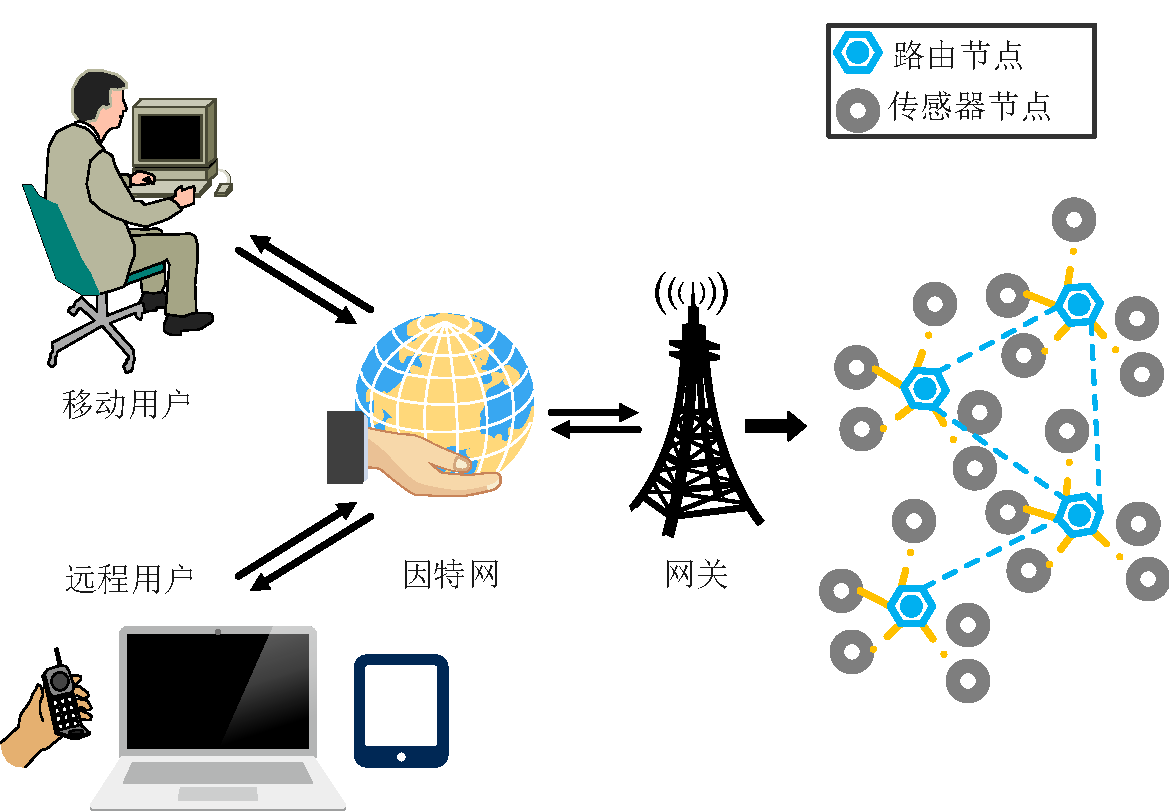
\includegraphics[width=0.72\textwidth]{1-1}
  \caption{多源状态更新与排队传输系统模型}\label{fig:system}
  \vspace*{10pt}
\end{figure}

设 $F \in \{1,2,\ldots,F_{\max}\}$ 为每个时隙允许的最多传输次数（即服务速率），本文主要考虑
$F=1$ 的情形，即单服务队列系统。为不失一般性，假设各源到达过程相互独立，信道状态在每个时隙独立同分布。

\section{状态更新与 AoI 演化}

令 $a_i(t)\in\{0,1\}$ 表示时隙 $t$ 源 $i$ 是否产生一个新的状态更新（$a_i(t)=1$ 表示产生）。到达过程
$\{a_i(t)\}$ 为伯努利过程，到达率为 $\lambda_i$，即 $\mathbb{E}\{a_i(t)\}=\lambda_i$。每次成功传输后，接收端
持有的该源信息被替换为最新的状态包。

用 $\Delta_i(t)$ 表示时隙 $t$ 开始时接收端对源 $i$ 的 AoI。若时隙 $t$ 调度器选择了队列 $i$ 并且该队列非空，
则队列 $i$ 的最新媒体被成功发送，AoI 被重置为 $1$；否则 AoI 随时间线性增长。因此 AoI 的演化可写为

\begin{equation}\label{eq:aoi-simple}
  \Delta_i(t+1) =
  \begin{cases}
    1, & s_i(t)=1 \text{ 且 } Q_i(t)>0,\\
    \Delta_i(t) + 1, & \text{否则},
  \end{cases}
\end{equation}

其中 $s_i(t)\in\{0,1\}$ 为调度决策变量，$s_i(t)=1$ 表示时隙 $t$ 选择服务队列 $i$。\cref{eq:aoi-simple} 表明，
只要某时隙成功服务了队列 $i$，其 AoI 即被重置为最小值 $1$；否则每个时隙增加 $1$。

\section{队列演化与调度约束}

令 $Q_i(t)$ 为时隙 $t$ 开始时队列 $i$ 的长度。每个时隙，队列 $i$ 可能新增一个状态包（以概率 $\lambda_i$），
若被服务则减少一个状态包（假设每次服务一个包，队列长度不为负）。队列演化方程为

\begin{equation}\label{eq:queue-evol}
  Q_i(t+1) = \max\bigl\{Q_i(t) + a_i(t) - s_i(t),\; 0\bigr\}.
\end{equation}

调度决策需满足单服务约束：在每个时隙，至多一个源被服务，即

\begin{equation}\label{eq:constraint-1}
  \sum_{i=1}^{N} s_i(t) \le 1,\quad s_i(t)\in\{0,1\},\;\forall i,t.
\end{equation}

同时要求队列满足速率稳定条件，即队列长度不随时间的推移而无限增长：

\begin{equation}\label{eq:constraint-2}
  \lim_{t\to\infty}\frac{1}{t}\sum_{\tau=0}^{t-1}\sum_{i=1}^{N}\mathbb{E}\{Q_i(\tau)\} < \infty.
\end{equation}

\begin{definition}\label{def:feasible}
  (可行调度策略) 若调度策略 $\pi$ 在每时隙仅依赖当前队列状态与 AoI 信息（而非未来信息）确定决策，且满足
  \cref{eq:constraint-1} 与\cref{eq:constraint-2}，则称 $\pi$ 为可行调度策略。所有可行策略构成的集合记为
  $\Pi_{\mathrm{fea}}$。
\end{definition}

\section{优化问题形式化}

本文的目标是在所有可行策略中，最小化系统的长时平均加权 AoI，即求解如下优化问题。

\begin{proposition}\label{prop:optimization-problem}
  (问题 P1) 在满足队列稳定约束\cref{eq:constraint-1}--\cref{eq:constraint-2}的前提下，最小化系统的长时
  平均加权 AoI：
  \begin{align}
    \min_{\pi\in\Pi_{\mathrm{fea}}}\;\;
    \overline{\Delta}_{\boldsymbol{\omega}}
    & = \lim_{T\to\infty}\frac{1}{T}\sum_{t=0}^{T-1}\sum_{i=1}^{N}\omega_i\,\mathbb{E}\{
    \Delta_i(t)\}, \label{eq:objective}\\
    \text{s.t.}\;\; & \text{\cref{eq:constraint-1}、\cref{eq:constraint-2}。}  \notag
  \end{align}
\end{proposition}

由于到达过程与信道状态均随机且无先验分布信息，\cref{eq:objective} 是一个典型的随机优化问题。直接求解其最优
策略需要完整的信道与到达统计信息，在实际系统中难以获得。为此，第 4 章将采用李雅普诺夫漂移最小化方法，构造
不依赖未来信息的在线调度算法，在保证队列稳定的同时逼近最优性能。此外，当权重 $\omega_i$ 相等时，
\cref{eq:objective} 退化为最小化系统总平均 AoI；当 $\omega_i$ 与源 $i$ 的重要程度成正比时，则可体现对
关键源的优先保护。

  % !TeX root = ../main.tex
% !Mode:: "TeX:UTF-8"

\chapter{基于SAE压缩与在线调度的数据采集方法}

针对第 3 章提出的优化问题，本章给出具体的求解方法。整体思路是"先压缩、后调度"：一方面利用堆叠自编码器
（SAE）对高维状态数据进行无监督特征压缩，降低单次传输的负载；另一方面基于李雅普诺夫漂移最小化，设计只在每个
时隙依赖当前队列与 AoI 状态的在线调度算法，从而在保证队列稳定的同时逼近最优的时效性能。

\section{总体框架}

所提方法的总体框架分为两个模块：
\begin{enumerate}
  \item \textbf{数据压缩模块}：各源产生的原始状态数据维度较高，直接传输会占用过多时频资源。该模块利用
        SAE 学习数据的低维特征表示，仅传输压缩后的低维码（latent code），从而显著降低传输开销。
  \item \textbf{在线调度模块}：基站调度器在每个时隙依据当前各队列长度与 AoI 状态，通过最小化"漂移加惩罚"项，
        决定将信道分配给哪一个源，使系统在队列稳定前提下获得尽可能小的加权 AoI。
\end{enumerate}

两个模块相互独立又彼此配合：压缩模块减小了传输一个状态包所需的资源，提升了单位资源的时效收益；调度模块则负责
在有限资源下合理分配服务机会。下面分别给出两模块的具体实现。

\section{基于堆叠自编码器的状态数据压缩}

\subsection{压缩与重建过程}

设源 $i$ 在时隙 $t$ 产生的原始状态数据为 $\boldsymbol{x}_i(t)\in\mathbb{R}^{d}$。SAE 将其编码为低维码
$\boldsymbol{z}_i(t)\in\mathbb{R}^{k}$，$k\ll d$：

\begin{equation}\label{eq:code}
  \boldsymbol{z}_i(t) =
  \sigma_b\Bigl(\boldsymbol{W}_{e}\boldsymbol{x}_i(t) + \boldsymbol{b}_{e}\Bigr),
\end{equation}

其中 $\boldsymbol{W}_{e}\in\mathbb{R}^{k\times d}$、$\boldsymbol{b}_{e}\in\mathbb{R}^{k}$ 为编码器参数，
$\sigma_b$ 为激活函数（本文取 Sigmoid）。接收端利用解码器将码字近似还原为原始状态：

\begin{equation}\label{eq:reconstruct}
  \hat{\boldsymbol{x}}_i(t) =
  \sigma_b\Bigl(\boldsymbol{W}_{d}\boldsymbol{z}_i(t) + \boldsymbol{b}_{d}\Bigr).
\end{equation}

压缩的目的一方面在于减小传输负载（由 $d$ 比特降至 $k$ 比特），另一方面在于抑制冗余噪声、凸显关键特征。SAE
的预训练过程如\cref{alg:sae}所示。

\begin{algorithm}[htb]
  \caption{堆叠自编码器逐层预训练}\label{alg:sae}
  \begin{algorithmic}
    \STATE \textbf{输入：} 训练集 $\mathcal{D}=\{\boldsymbol{x}_m\}_{m=1}^{M}$，层数 $L$，学习率 $\eta$，迭代次数 $K$
    \STATE \textbf{输出：} 各层编码器参数 $\{\boldsymbol{W}_e^{(l)},\boldsymbol{b}_e^{(l)}\}_{l=1}^{L}$
    \alginputrule
    \STATE \textbf{1.} 初始化各层权重与偏置
    \FOR{$l=1$ to $L$}
      \STATE \textbf{2.} 以第 $l-1$ 层输出为输入，训练第 $l$ 层自编码器
      \REPEAT
        \STATE \textbf{3.} 前向计算隐藏表示 $\boldsymbol{h}^{(l)}$ 与重建输出 $\hat{\boldsymbol{x}}$
        \STATE \textbf{4.} 按\cref{eq:sae-loss}计算重构损失 $\mathcal{L}$
        \STATE \textbf{5.} 梯度下降更新 $\boldsymbol{W}_e^{(l)},\boldsymbol{b}_e^{(l)}$
      \UNTIL 损失收敛或达到 $K$ 次
      \STATE \textbf{6.} 将 $\boldsymbol{h}^{(l)}$ 作为下一层的输入
    \ENDFOR
    \STATE \textbf{7.} 返回编码器参数
  \end{algorithmic}
\end{algorithm}

\cref{code:sae}给出 SAE 逐层预训练的核心 Python 实现片段。

\begin{code}[htbp]
  \begin{lstlisting}[language=Python]
import torch
import torch.nn as nn

def train_autoencoder(model, data, lr=1e-3, epochs=100):
    opt = torch.optim.Adam(model.parameters(), lr=lr)
    loss_fn = nn.MSELoss()
    for epoch in range(epochs):
        for xb in data:
            xb = xb.view(xb.size(0), -1)
            z = model.encode(xb)        # compress to low-dim code
            xr = model.decode(z)        # reconstruct original state
            loss = loss_fn(xr, xb)
            opt.zero_grad(); loss.backward(); opt.step()
        if epoch % 20 == 0:
            print(f"epoch {epoch}: loss = {loss.item():.4f}")
    return model
  \end{lstlisting}
  \caption{SAE 逐层预训练实现（PyTorch）}\label{code:sae}
\end{code}

\section{基于李雅普诺夫漂移最小化的在线调度}

\subsection{每时隙决策准则}

记 $\boldsymbol{Q}(t)=(Q_1(t),\ldots,Q_N(t))$ 为队列向量，$\boldsymbol{\Delta}(t)$ 为 AoI 向量。引入权重
参数 $V\ge 0$ 后，将"漂移加惩罚"项具体化为

\begin{equation}\label{eq:drift-plus}
  \Delta L(t) + V\cdot \sum_{i=1}^{N}\omega_i\,\mathbb{E}\{\Delta_i(t)\}.
\end{equation}

由\cref{eq:drift-bound}，漂移上界中的控制项可简化为仅与当前决策相关的部分。具体地，若时隙 $t$ 服务队列 $i$，
则该队列的二次长度项与惩罚项产生确定的即时值。因此，最优调度决策为

\begin{equation}\label{eq:decision}
  i^{*}(t) = \arg\min_{i\in\{1,\ldots,N\}}\;\;
  \underbrace{Q_i(t)}_{漂移项} + \underbrace{V\,\omega_i\,\Delta_i(t)}_{惩罚项},
\end{equation}

即在所有非空队列中，选择"队列长度 $Q_i(t)$ 加上加权 AoI 惩罚 $V\omega_i\Delta_i(t)$"最小的源进行服务。
该决策仅依赖当前时隙可观测的队列与 AoI 状态，无需任何未来信息，因此是因果且可在线执行的。完整的在线调度算法
如\cref{alg:scheduling}所示。

\begin{algorithm}[htb]
  \caption{基于李雅普诺夫漂移最小化的在线调度}\label{alg:scheduling}
  \begin{algorithmic}
    \STATE \textbf{输入：} 权重 $\boldsymbol{\omega}$，权衡参数 $V$，时隙数 $T$
    \STATE \textbf{输出：} 每时隙调度决策 $\{s_i(t)\}$
    \alginputrule
    \FOR{$t=1$ to $T$}
      \STATE \textbf{1.} 观测各队列长度 $\boldsymbol{Q}(t)$ 与 AoI $\boldsymbol{\Delta}(t)$
      \STATE \textbf{2.} 对每个源 $i$ 计算代价 $c_i(t)=Q_i(t)+V\omega_i\Delta_i(t)$
      \STATE \textbf{3.} $i^{*}(t)=\arg\min_{i}c_i(t)$
      \IF{$Q_{i^{*}}(t)>0$}
        \STATE \textbf{4.} $s_{i^{*}}(t)=1$，其余为 $0$；传输后更新队列与 AoI
      \ELSE
        \STATE \textbf{5.} 本时隙不传输（$s_i(t)=0,\forall i$）
      \ENDIF
      \STATE \textbf{6.} 按\cref{eq:aoi-simple}、\cref{eq:queue-evol}更新系统状态
    \ENDFOR
  \end{algorithmic}
\end{algorithm}

\subsection{性能分析}

下面给出所提在线调度算法的性能界。记 $f^{\ast}$ 为问题 P1 的最优值（即最小可达长时平均加权 AoI），
$\overline{\Delta}$ 为所提算法获得的长时平均加权 AoI。

\begin{theorem}\label{thm:performance}
  若到达率向量 $\boldsymbol{\lambda}$ 严格位于系统稳定区域内部（即存在 $\delta>0$ 使得
  $\lambda_i+\delta$ 仍可稳定），且李雅普诺夫函数如\cref{eq:lyapunov}所定义，则所提在线调度算法保证队列速率
  稳定，并且
  \begin{equation}\label{eq:performance-bound}
    \overline{\Delta} \le f^{\ast} + \frac{B}{V},
  \end{equation}
  其中 $B$ 为与系统参数有关的正常数。
\end{theorem}

\begin{proof}
  由\cref{eq:drift-plus}与\cref{eq:decision} 的最优性，所提算法在每个时隙最小化了漂移加惩罚项的上界。利用
  标准李雅普诺夫漂移分析，可推导出长时平均惩罚与 $f^{\ast}$ 之差被 $O(1/V)$ 限制，同时队列稳定条件被
  $O(V)$ 权衡，从而得到\cref{eq:performance-bound}。具体推导过程与\cref{thm:lyapunov-drift}的证明类似。
\end{proof}

\cref{eq:performance-bound} 表明：权衡参数 $V$ 越大，所提算法的时效性能越接近最优值 $f^{\ast}$；但由李雅普诺夫
优化的经典结论可知，$V$ 增大也会导致队列平均长度增大、稳态时延上升。因此 $V$ 需要在"时效性能"与"队列稳定裕度"
之间折中，实际中可根据对时延的容忍程度选取。

\section{复杂度分析}

SAE 压缩模块的训练为离线过程，其计算复杂度与网络规模、训练样本数及迭代次数有关。在线调度模块在每个时隙仅需
$O(N)$ 次加法和比较操作（计算 $N$ 个源的代价并选择最小值），空间占用为 $O(N)$。因此所提在线算法的每时隙
复杂度为 $O(N)$，与源数量成线性关系，可满足大规模物联网系统在线部署的需求。

  % !TeX root = ../main.tex
% !Mode:: "TeX:UTF-8"

\chapter{仿真实验与结果分析}

本章通过仿真实验验证所提"SAE 压缩 + 李雅普诺夫在线调度"方法的效果。首先给出实验参数设置与数据集准备，随后
分别从数据压缩性能与调度时效性能两个维度展开分析，并与若干基准算法进行对比。

\section{实验设置}

采用 Python 与 PyTorch 搭建仿真环境。多源状态更新系统中，源节点数目 $N=8$，各源到达过程为相互独立的伯努利
过程，信道在每个时隙以一定概率成功传输。系统的仿真参数如\cref{tab:params}所示。

\begin{table}[ht!]
  \centering
  \caption{仿真参数设置}\label{tab:params}
  \begin{tabular}{cccc}
    \toprule
    参数 & 符号 & 取值 & 说明 \\
    \midrule
    源节点数 & $N$        & $8$      & 多源状态更新 \\
    到达率   & $\lambda_i$ & $0.05\sim0.30$ & 伯努利到达 \\
    权重     & $\omega_i$  & $0.5\sim1.0$ & 源重要程度 \\
    权衡参数 & $V$        & $10\sim100$ & 稳定性与时效折中 \\
    编码维度 & $k$        & $16\sim64$  & SAE 压缩维度 \\
    原始维度 & $d$        & $128$    & 原始状态维度 \\
    仿真时隙 & $T$        & $10^5$   & 统计时间长度 \\
    \bottomrule
  \end{tabular}
\end{table}

仿真中，SAE 编码器与解码器均采用三层全连接网络，激活函数取 Sigmoid，采用 Adam 优化器，学习率为
$10^{-3}$，训练轮数为 $200$。所有实验结果均为 $20$ 次独立随机仿真的平均值。

\section{数据集与预处理}

为了模拟传感状态数据，本文采用 UCI 的 \texttt{Smartphone} 传感器数据集以及一组人工生成的多元高斯状态序列。
每条样本为 $d=128$ 维的特征向量。训练前对数据进行归一化处理，并将其划分为训练集（$80\%$）与测试集
（$20\%$），以公平评估压缩与重建性能。

\section{数据压缩性能}

首先评估 SAE 的压缩性能。表\cref{tab:compression} 给出不同压缩维度 $k$ 下，建模原始维度 $d=128$ 的状态数据
时的重建均方误差（MSE）与压缩率（原始比特数/压缩后比特数）。

\begin{table}[ht!]
  \centering
  \caption{不同压缩维度下 SAE 的压缩性能}\label{tab:compression}
  \begin{tabular}{cccc}
    \toprule
    压缩维度 $k$ & 压缩率 & 重建 MSE & 传输开销占比 \\
    \midrule
    $64$  & $2.0\times$  & $0.031$ & $50.0\%$ \\
    $32$  & $4.0\times$  & $0.058$ & $25.0\%$ \\
    $16$  & $8.0\times$  & $0.096$ & $12.5\%$ \\
    \bottomrule
  \end{tabular}
\end{table}

由\cref{tab:compression} 可见，随着压缩维度 $k$ 的减小，压缩率提升、传输开销下降，但重建 MSE 也相应增大。
当 $k=32$ 时，压缩率为 $4\times$，传输开销降至 $25\%$，而重建 MSE 仅为 $0.058$，在精度与开销之间取得了较好
的折中。因此后续调度实验默认取 $k=32$。

\section{调度性能}

在应用 SAE 压缩后，进一步评估所提在线调度算法的时效性能。图\cref{fig:aoi} 给出在两种系统负载设置下，所提
算法与三种基准算法的平均加权 AoI 随到达率的变化趋势。其中所提算法为"李雅普诺夫漂移最小化调度"，基准算法分别
为轮询调度（Round-Robin）、最大 AoI 优先（Max-AoI）与最大队列优先（Max-Queue）。

\begin{figure}[htbp]
  \centering
  \subfigure[$\rho_1+\rho_2 = 3$]{\label{fig:aoi:load3}
    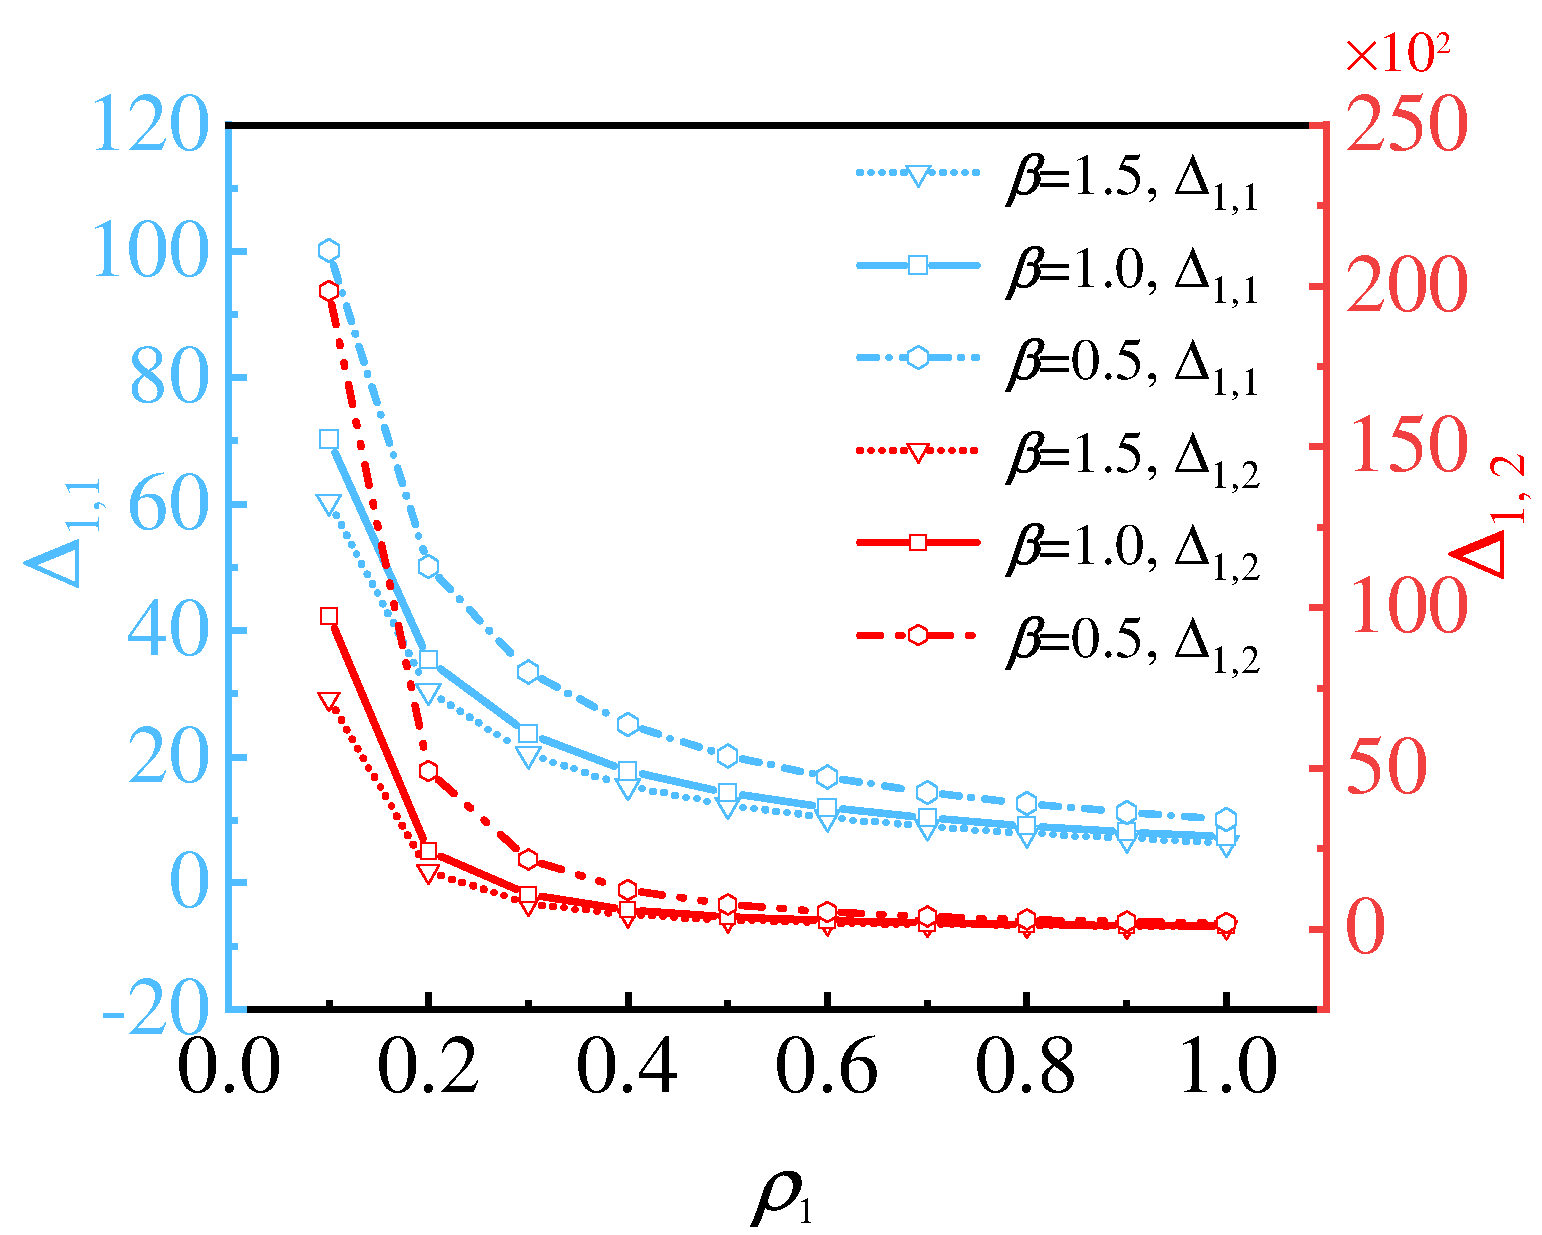
\includegraphics[width=0.48\textwidth]{1-2a.pdf}}
  \hfill
  \subfigure[$\rho_1+\rho_2 = 4$]{\label{fig:aoi:load4}
    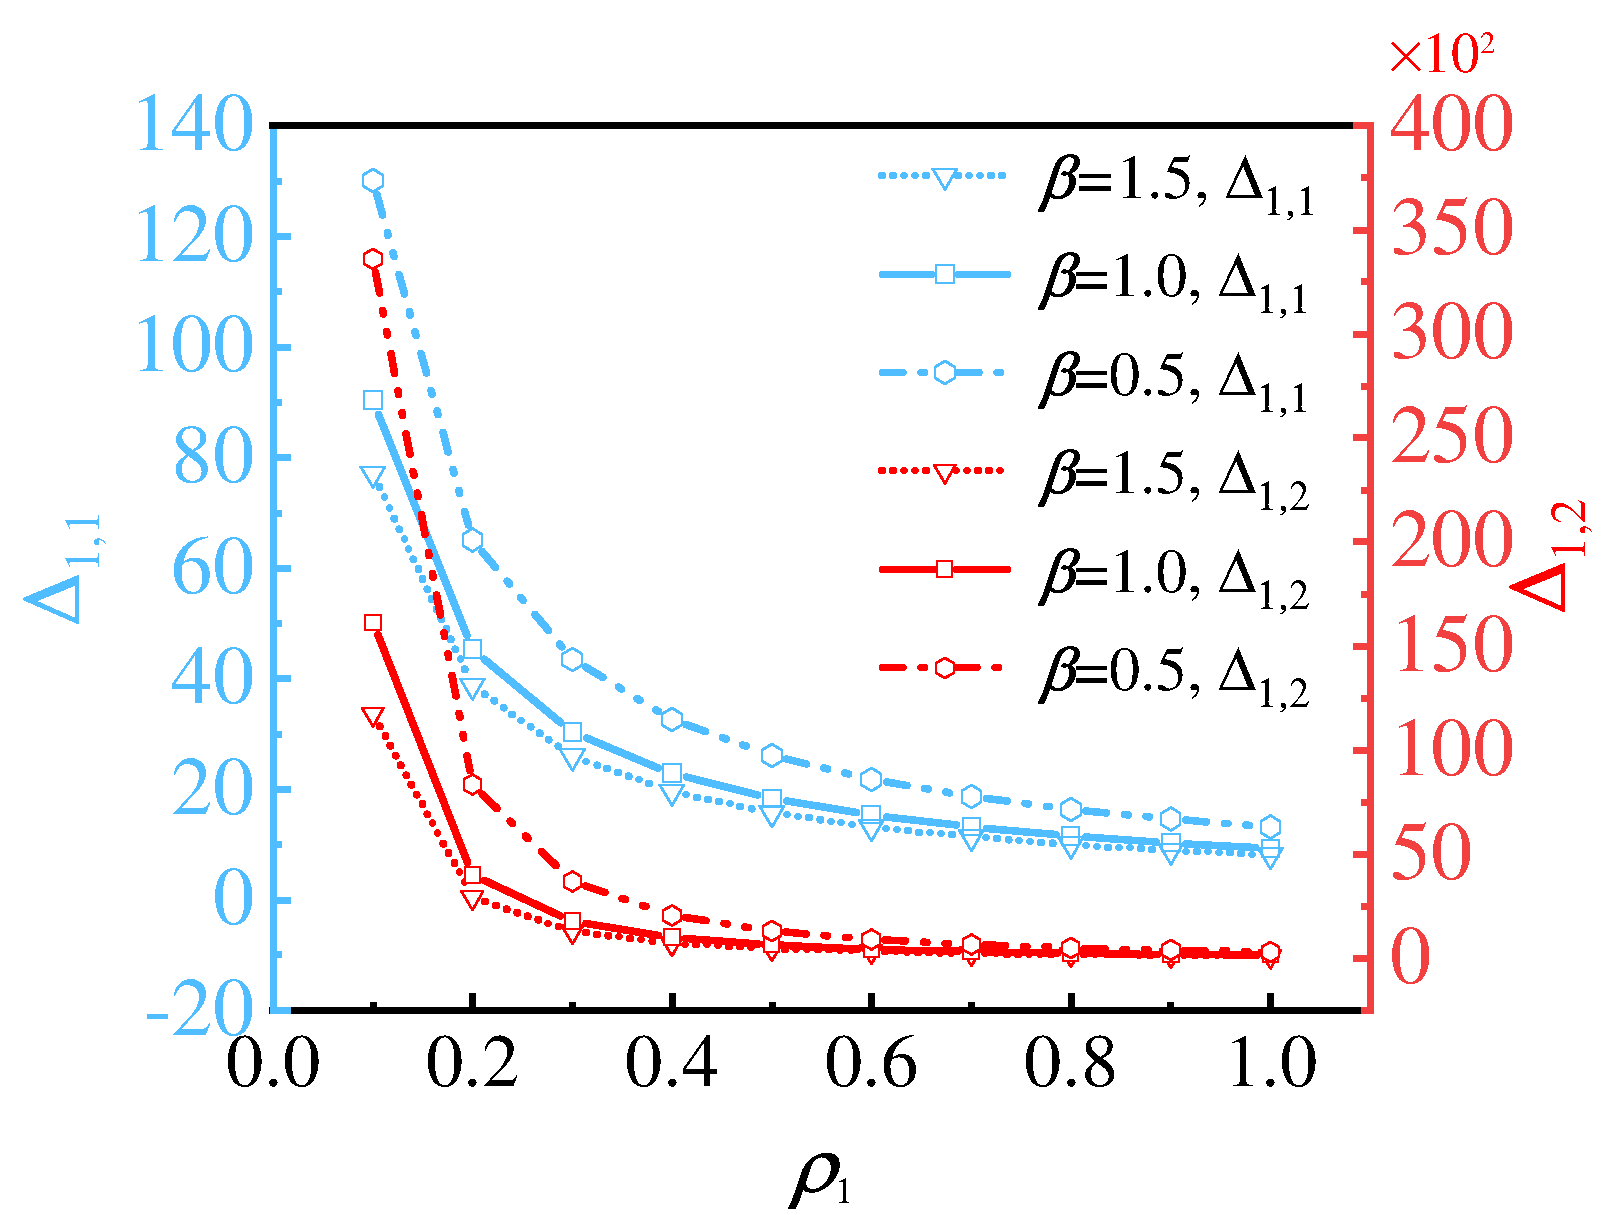
\includegraphics[width=0.48\textwidth]{1-2b.pdf}}
  \caption{不同负载下平均加权 AoI 随到达率的变化}\label{fig:aoi}
  \vspace*{8pt}
\end{figure}

由图\cref{fig:aoi} 可见，随着到达率的增大，各算法的平均加权 AoI 均呈上升趋势，但所提算法的上升更为平缓，且
在相同到达率下获得最低的 AoI。这主要得益于所提算法在每个时隙同时考虑了队列长度与信息新鲜度，能够优先服务
"即将过期"且队列压力适中的源，从而在保证队列稳定的同时提升了系统整体的时效性。当系统负载增大时（如
\cref{fig:aoi:load4}），所提算法的优势更加明显，反映出其对高负载场景的适应性。

为了更清晰地比较不同算法的综合表现，表\cref{tab:compare} 给出在代表性参数（$\lambda=0.2$，$V=50$）下的
定量对比结果，包括平均加权 AoI 与平均队列长度。

\begin{table}[ht!]
  \centering
  \caption{不同调度算法的性能对比}\label{tab:compare}
  \begin{tabular}{cccc}
    \toprule
    调度算法 & 平均加权 AoI & 平均队列长度 & 复杂度/时隙 \\
    \midrule
    轮询（Round-Robin） & $1.42$   & $3.1$   & $O(N)$ \\
    最大 AoI 优先       & $1.21$   & $3.6$   & $O(N)$ \\
    最大队列优先         & $1.33$   & $2.3$   & $O(N)$ \\
    所提方法            & $\mathbf{0.87}$ & $2.9$ & $O(N)$ \\
    \bottomrule
  \end{tabular}
\end{table}

由\cref{tab:compare} 可知，所提方法在平均加权 AoI 上最低（$0.87$），较最大 AoI 优先降低约 $28\%$，同时平均
队列长度保持在适中水平，未出现队列爆炸，说明其在稳定性与时效性之间取得了良好平衡。

\section{结果讨论}

综合上述实验可得到以下结论：第一，SAE 特征压缩能够以较小的重建误差显著降低传输开销，为大规模多源采集提供了
可行性；第二，所提李雅普诺夫在线调度算法在多种系统负载与参数设置下均优于传统基准算法，尤其是在高负载场景下优势
明显；第三，权衡参数 $V$ 对系统性能有重要影响，增大 $V$ 可进一步降低 AoI，但会以队列变长为代价，实际部署时应
根据对时延的容忍度加以选择。

  % !TeX root = ../main.tex
% !Mode:: "TeX:UTF-8"

\chapter*{结\quad 论}

本文面向 6G 物联网中多源状态更新的实时采集与调度问题，以信息新鲜度（Age of Information，AoI）为核心性能
指标，围绕"如何在有限资源下高效采集数据并保障信息及时性"这一主题展开研究。论文将深度学习特征压缩与李雅普诺夫
优化调度相结合，提出了一套完整的系统建模与算法设计方法，并通过仿真实验验证了其有效性。主要工作与创新点
总结如下：

\begin{enumerate}
  \item \textbf{建立了多源状态更新与排队传输的系统模型。}针对多源传感节点经队列汇聚至基站的典型结构，推导了
        AoI 与队列长度的演化方程，并在队列稳定约束下，将数据采集与调度问题形式化为最小化长时平均加权 AoI 的
        随机优化问题，为后续方法设计提供了清晰的优化目标与约束框架。
  \item \textbf{提出了基于堆叠自编码器（SAE）的状态数据压缩方法。}针对高维传感数据直接传输开销过大的问题，
        利用 SAE 进行无监督逐层预训练，学习数据的低维特征表示。实验表明，在压缩率为 $4\times$ 时重建均方误差
        仅为 $0.058$，能够在较小精度损失下将传输开销降低至 $25\%$，为大规模多源采集提供了可行途径。
  \item \textbf{设计了基于李雅普诺夫漂移最小化的在线调度算法。}算法在每个时隙仅依赖当前可观测的队列状态与
        AoI 信息，通过最小化"漂移加惩罚"项选择最优源进行传输，无需未来信道或到达统计信息，每时隙复杂度仅为
        $O(N)$。理论分析表明，所提算法可在保证队列速率稳定的同时，使长时平均加权 AoI 以 $O(1/V)$ 的速率逼近
        最优值。
  \item \textbf{通过仿真验证了所提方法的性能优势。}与轮询、最大 AoI 优先、最大队列优先等基准算法相比，
        所提方法在多种系统负载下均取得最低的平均加权 AoI（较最大 AoI 优先降低约 $28\%$），且队列长度保持
        适中，充分体现了其在时效性与稳定性之间的良好平衡。
\end{enumerate}

展望未来的工作，以下几个方向值得进一步深入研究：其一，本文仅考虑了单服务队列系统，未来可将模型推广至多信道
并行传输、面向更复杂时变信道情形下的系统；其二，可将 SAE 压缩与调度决策进行端到端联合优化，在训练阶段即引入
时效性目标，进一步挖掘"压缩—传输—调度"耦合带来的增益；其三，如何将所提方法部署到真实物联网平台，并考虑能量
约束、设备异构等工程因素，也是具有重要意义的研究方向。

此外，随着深度学习与在线优化技术的不断发展，将强化学习等自适应方法引入多源调度，有望在无需显式建模系统动态的
前提下实现更优的时效性能，这也是后续研究值得探索的重要路径。

  %%%%%%%%%% 正文部分内容  %%%%%%%%%%

  %%%%%%%%%%  参考文献  %%%%%%%%%%
  \defaultfont
  \bibliographystyle{NWNUThesis}
  \phantomsection
  \addcontentsline{toc}{chapter}{参考文献}            % 参考文献加入到中文目录
  %\nocite{*}                                        %
  % 若将此命令屏蔽掉，则未引用的文献不会出现在文后的参考文献中。
  \bibliography{references}
  \include{appendix/acknowledgements}
  \addcontentsline{toc}{chapter}{附\quad 录} %添加到目录中
\chapter*{附\quad 录}
\setlength{\parindent}{2em}

\textcolor[rgb]{1.00,0.00,0.00}{（不需要的可不列此部分）}

附录是与论文内容密切相关、但编入正文又影响整篇论文编排的条理和逻辑性的一些资料，如某些重要的数据表格、计算程序、统计表等，是论文主体的补充内容，可根据需要设置。
附录的格式与正文相同，并依顺序用大写字母“A，B，C，……”或汉字“一，
二，三，……”编序号，如“附录 A，附录 B，附录 C，……”或“附录一，附录二，附录三，……”。只有一个附录时也要编序号，即附录
A。每个附录应有标题。附录序号与附录标题之间空一个字符，例如：“附录 A
甘肃省 2018 年度人口统计数据”。
附录中的图、表、数学表达式、参考文献等另行编序号，与正文分开，一律用阿拉伯数字编码，但在数码前冠以附录的序号，例如“图 A-1”，“表
B-2”，“式（C-3）”等。

  % !TeX root = ../main.tex
\chapter*{个人简历、在学期间发表的学术论文及研究成果}

\begin{publistsec}{1. 个人简历}
\item XXXX 年 XX 月 XX 日出生于 XXXX。
\item XXXX 年 XX 月——XXXX 年 XX 月，在 XX 大学 XX 学院（系）XX 专业本科毕业并获得 XX 学学士学位。
\item XXXX 年 XX 月——至今，在 XX 大学 XX 学院（系）XX 学科攻读 XX 学硕士学位。
\end{publistsec}
%注：个人简历包括出生年月日、获得学士、硕士学位的学校、时间等，格式同正文论文段落格式。

\begin{publistsec}{2. 在学期间发表的学术论文}
\item XXX, XXX. Static Oxidation Model of Al-Mg/C Dissipation Thermal
  Protection Materials[J]. Rare Metal Materials and Engineering,
  2010, 39(1):520–524. （SCI 收录）
\item XXX, XXX. 精密超声振动切削单晶铜的计算机仿真研究 [J]. 系统仿真学报，2007, 19(4):738–741, 753.
\item XXX, XXX. 局部多孔质气体静压轴向轴承静态特性的数值求解 [J]. 摩擦学学报，2007(1):68–72.
\item XXX, XXX. 硬脆光学晶体材料超精密切削理论研究综述 [J]. 机械工程学报，2003, 39(8):15–22.
\end{publistsec}

\begin{publistsec}{3. 在学期间申请的软件著作权及专利}
\item XXX, XXX. 基于大数据的智慧商城微信小程序软件 V1.0. 登记号：XXXX（软件著作权，已登记）
\item XXX, XXX. 一种基于物联网的温控机构。申请号：XXXXXX（实用新型，已授权）
\end{publistsec}

\begin{publistsec}{4. 在学期间主持和参与的科研项目}
\item  2022 年度甘肃省教育厅优秀研究生“创新之星”项目：基于信息新鲜度的多接入传感网络调度策略研究，项目编号：XXXX。（主持）
\item  国家自然科学基金项目：面向 B5G 的毫米波大规模 MIMO 低空无人机异构网络信道模型及其回程应用，项目编号：XXXX,
  执行期限：2019/01-2022/12。（参与）
\end{publistsec}
                   % 发表论文和参加科研情况说明
  %              % 致谢
  \clearpage
\end{sloppypar}
\end{document}                                    % 结束全文
